\documentclass[
utf8,%     More capable input encoding than latin-1.
parskip,%  For vertical whitespace between paragraphs.  This comes down to more than just using parskip.sty, so it's better to use this class option.
% S5MP % If you intend to really use margin paragraphs (not recommended!).
%  crop,%     Produce output with crop marks and paper size A4.  Liu-Tryck should like this.  Automatically adds information, including the physical page number, at the top of each page.
%     Add option 'noInfo' to suppress the info at the top of each page when using option 'crop'.
% Font options: 'kp' (default), 'times', 'lm'.  The KpFonts (loaded using 'kp'), is the most complete font among the provided options.  Among other, it supports slanted small caps.  See rtthesis.cls for more details regarding the font options.
largesmallcaps,intlimits,widermath,% Good options to KpFonts.
sharecounter,nobreak,definition=marks,%  See comments in the results chapter of this document for more information on these options!
%numbers, % If you want to cite references by numbers, use this option.
noparts% Use option 'noparts' if you do not make use of part divisions.
]{rtthesis}

\usepackage{mythesis}
\usepackage[outdir=./]{epstopdf}
\usepackage{algorithm}
\usepackage{algpseudocode}
\usepackage{pdfpages}

\let\cross\times
\let\vec\boldsymbol

\begin{document}
  \setlength\parindent{0pt}

  \selectlanguage{english}
  \makeFrontPage
  \frontmatter
  \maketitle
  \makeLibraryPage{Rigid body physics on the GPU using spherical voxelization.
}

  %\begin{abstract}[swedish]
  %  Rigid body physics on the GPU using spherical voxelization.

  %\end{abstract}
  %\begin{abstract}[english]
  %  If your thesis is written in English, the primary abstract would go here while the Swedish abstract would be optional.

  %\end{abstract}

  %\begin{acknowledgments}
  

  \addvspace{1em}
  \begin{flushright}
    \textit{%
      Linköping, Januari 2020\\
      N N och M M%
    }
  \end{flushright}
\end{acknowledgments}

  \tableofcontents
  %\begin{notation}% Passing the option "old" to the notation environment will redefine the notationtabular environment so that it produces an old style LaTeX tabular instead of a ctable.sty style tabular.
  \centering

  \begin{notationtabular}{Några mängder}{Notation}{Betydelse}
    $\naturals$ & Mängden av naturliga tal \\
    $\reals$ & Mängden av reella tal \\
    $\complexes$ & Mängden av komplexa tal \\
  \end{notationtabular}

  \begin{notationtabular}{Förkortningar}{Förkortning}{Betydelse}
    \abbrARMA\index{ARMA@\abbrARMA!abbreviation} & Auto-regressive moving average \\
    \abbrPID\index{PID@\abbrPID!abbreviation} & Proportional, integral, differential (regulator) \\
  \end{notationtabular}
\end{notation}


  \mainmatter
  \raggedbottom

  \chapter{Introduction}\label{cha:intro}

\section{Motivation}

Synthetic data generation is a subject with increasingly high relevance.
The data can be used for training and validation of self-learning systems,
something which is becoming increasingly more popular and useful within vision
based problems. Solving methods for high speed generation of these datasets
can greatly increase the productivity and development of these
types of algorithms.

\section{Purpose}

For the purpose of generating synthethic data this thesis will investigate the use of physics
simulation for part distribution. The situation investigated in this thesis
is when several, identical models is  'poured' into a bin and simulated for their
final resting distribution. In figure~\ref{fig:plb}, the situation
the thesis aims to simulate is visualized. Only the distribution of the parts
will be simulated, i.e. the robotic arm and gripper used for picking the parts will not be simulated. For these simulations
performance is of high interest as generation of large amounts of data generation
is one of the key aspects. Due to the interest for performance a GPU method will
be investigated and compared to a more traditional CPU based solution.

\begin{figure}[ht]
  \centering
  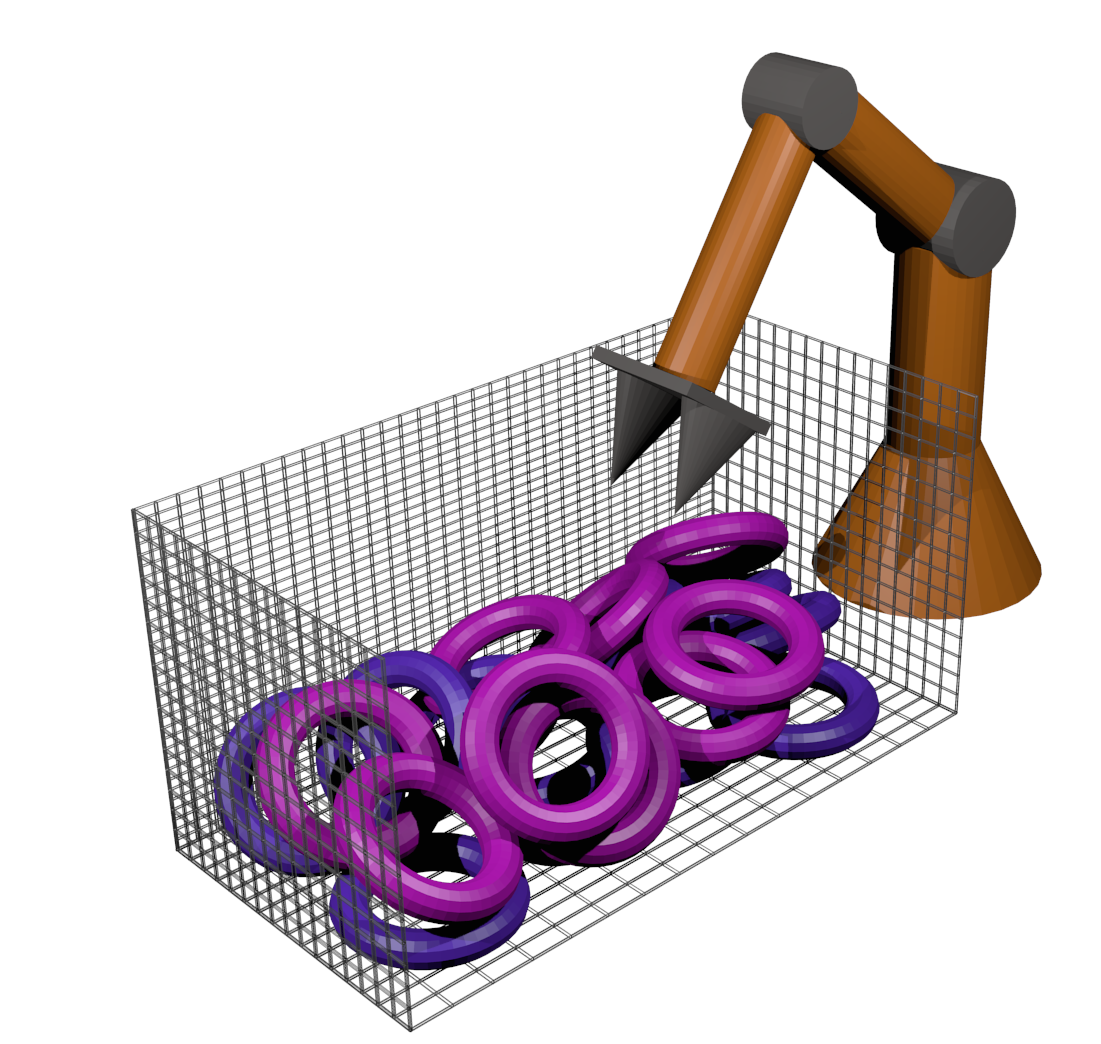
\includegraphics[width = 0.8\textwidth]{binBlender.png}
  \caption{The situation which the thesis aims to simulate.}
  \label{fig:plb}
\end{figure}

\section{Problem Statement}
How can a GPU rigid body solver be realised and used for synthetic data generation
 and how does it compare against Bullet?

\section{Limitations}
Since the system is somewhat chaotic in nature, deviations from a high accuracy
simulation in exchange for performance is accepted. The simulation should be reasonable
and the final distribution must be valid. For instance a detailed
model for the friction might not grant a better final distribution than a simple one.
Additional limitations are hardware. The methods will be evaluated on the hardware
provided by SICK IVP. Graphics card: GeForce GTX 960 with 4 GB GDDR5 VRAM.
CPU: Intel Xeon W3530 at 2.8 GHz.
Memory: 6 GB RAM.

Initially the Rigid-body GPU pipeline of Bullet 3.x was to be investigated, however
it has become apparent that the implementation was more or less abandoned in 2013
when Erwin Coumans started working for Google instead of AMD. While operational,
no API for it exists. Due to it's state it is excluded from the thesis.
A self-implemented GPU rigid body solver will be implemented and compared to Bullet.

\section{Methodology}
Validation for physics simulations is a very difficult topic. Since the aim for
the thesis is to produce realistic enough distributions we do not need to focus
on absolutely realistic results but can instead evaluate the results in terms of
a few key properties. Of interest are: performance, since the more images
that can be generated the better the chances of finding rare problems; correctness,
as the simulations need to be relatively correct to give rise to the problems that
 happen in real life scenarios; concave collision, since the objects might
 be concave and contain holes or other cavities.

The methods will be evaluated in a comparative fashion against one another.

Two CPU methods, the rectangle bounding-box and HACD will be implemented using
BulletPhysics 2.83, an open-source, permissively licensed, optimized game physics
library. The third method will be a GPU method implemented from scratch using a
voxelized particle method with impulses.

  \chapter{Theory}\label{cha:theory}
This chapter describes the fundamentals of the equations needed to perform physics simulations.
\section{Rigid body dynamics}
According to~\cite{baberrigid} there are three major methods for solving rigid body
dynamics; penalty methods, impulse methods and constraint based methods.
In common with most methods for rigid body dynamics is the need for the governing laws of
motion which move the simulation forward in time. In addition methods for collision detection
and collision response is needed. The planned use of a GPU collision
detection will be limited to a uniform grid/sort-based method, as described by~\cite{gpugems}.
The methods of using mass splitting and spherical decomposition are very similar
to what~\cite{flex} and~\cite{bulletPipeline} have presented with regards to
constraint based physics. This thesis will describe a method for using it with
impulse based physics while keeping the calculations on the GPU. The laws of motion and relevant vectors and variables
for updating the states of the bodies are summarized in figure~\ref{fig:diag}.
Subindices $a$ and $b$ refer to which body the variable belong to.
The variables used are; velocity, $v$; rotational velocity, $\omega$; vector to
the collision point, $r$; mass, $m$; collision normal, $n$ and inertia tensor, $I$.

\begin{figure}[H]
  \centering
  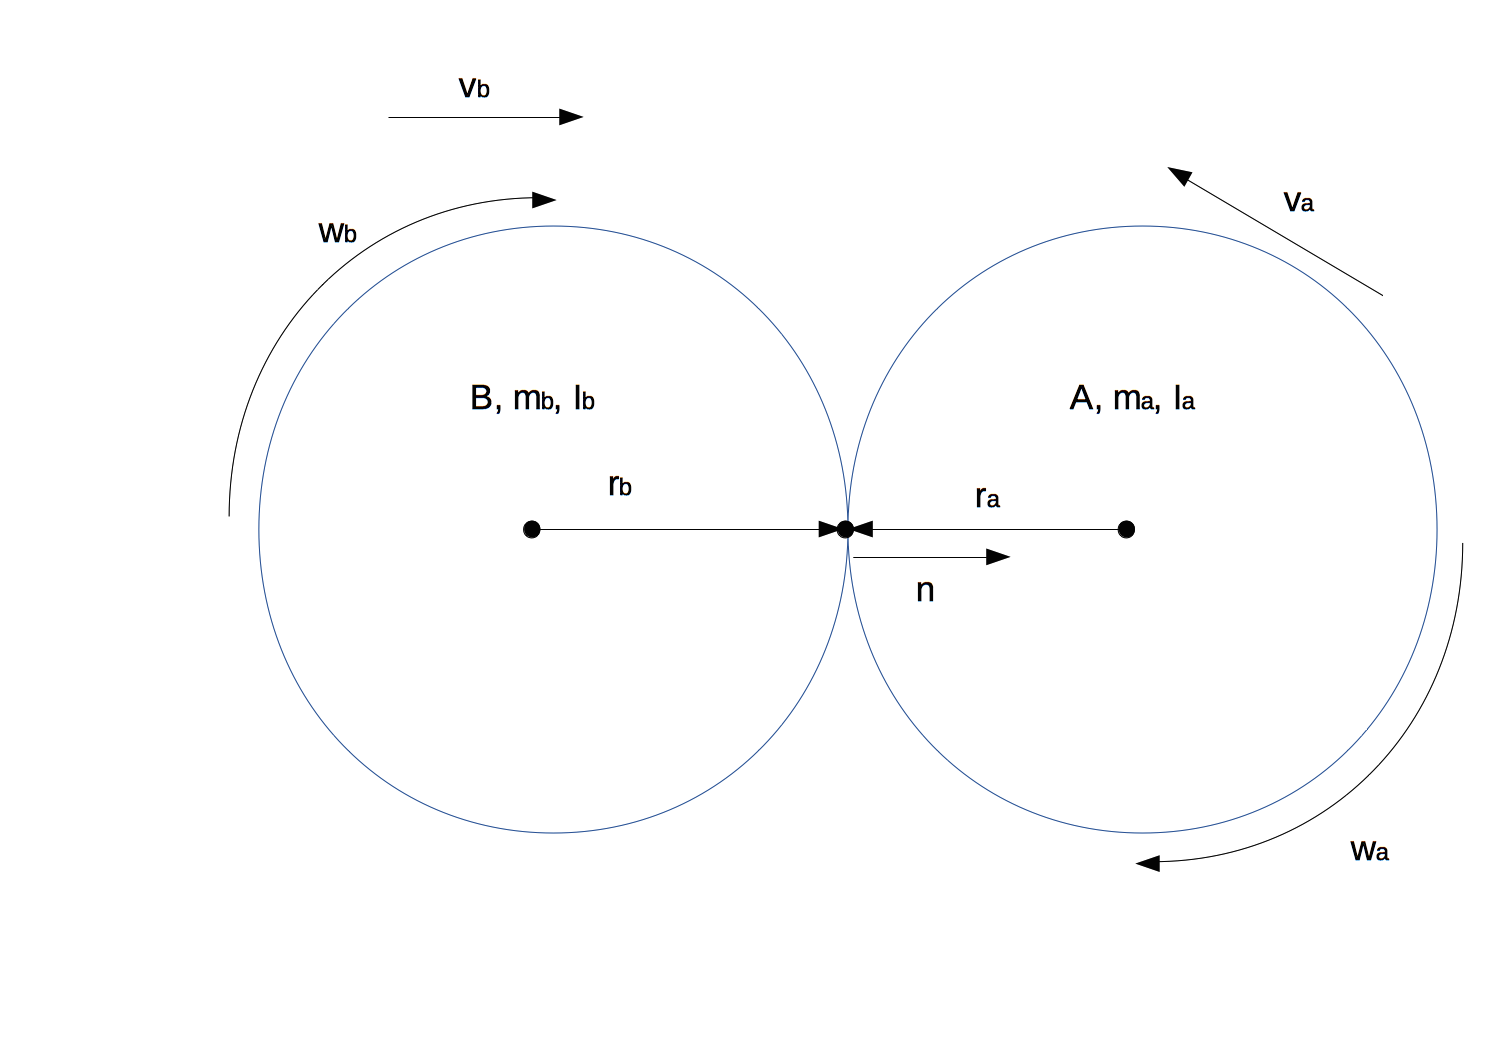
\includegraphics[width = 0.8\textwidth]{physicsscheme.png}
  \caption{Diagram of the relevant vectors and variables used when resolving a collision. Variables used are; velocity, $v$; rotational velocity, $\omega$; vector to
  the collision point, $r$; mass, $m$; collision normal, $n$ and inertia tensor, $I$.
   Subindices $a$ and $b$ refer to which body the variable belong.}
  \label{fig:diag}
\end{figure}

\subsection{Laws of motion}
The following equations govern the motions of rigid bodies are summarized by~\cite{hansson}. They are repeated here for reference.
Here $\vec{P}$ refer to the the linear moment, $\vec{L}$ refer to the angular
moment and $\vec{I}$ the inertia tensor of the body, expressed in the mass center of the body.

\begin{equation}
  \frac{d\vec{P}}{dt}=m\frac{d\vec{v}}{dt} = \vec{f}
\end{equation}

\begin{equation}
  \frac{d\vec{L}}{dt}=\vec{I}\frac{d\vec{\omega}}{dt} = \vec{\tau}
\end{equation}

\begin{equation}
  \frac{d\vec{x}}{dt}=\vec{v}
\end{equation}

\begin{equation}
  \frac{d\vec{q}}{dt} = \frac{1}{2}\vec{\omega}\vec{q}
\end{equation}

\begin{equation}
  \vec{I} = \vec{R}\vec{I}_0\vec{R}^T
\end{equation}

\subsection{Integrating the laws of motion discretely}
The equations in the previous subsection need to be calculated in discrete time steps.
For this purpose we need a discrete integration technique. The
simplest among them is the Euler step. With a fixed time step, $\Delta t$,
equations~\ref{eq:1}~to~\ref{eq:2} can be used to move the simulation one step forward in time.
The update for the quaternions are based on the description given by~\cite{fossum}.

\begin{equation}\label{eq:1}
  \vec{v}_{t + \Delta t} = \vec{v}_{t}+\frac{\vec{P}}{m}
\end{equation}
\begin{equation}
  \vec{L}_{t + \Delta t} = \vec{L}_{t}+\vec{\tau}\Delta t
\end{equation}

\begin{equation}
  \vec{\omega}_{t + \Delta t} = \vec{w}_t+\vec{I}^{-1}\vec{\tau}\Delta t
\end{equation}

\begin{equation}\label{eq:2}
  \vec{x}_{t + \Delta t} = \vec{x}_{t} + \vec{v}_t\Delta t
\end{equation}

\section{Impulse method}\label{sec:imp}
To use the impulse method we need to solve the impulse $\vec{j}$. ~\cite{baraff} explains the details
and derivations of the results below, and it is recommended that the interested reader look through
his work.

Solving physics using the impulse method has the benefit of having few external tuning
parameters. In the suggested implementation tuning parameters could be; $\Delta t$, the time step;
$\mu$, the friction coefficient, and the bias factor which is explained further in section~\ref{sec:bias}.

The following equation can be used to calculate the impulse created in the
collision between body A and body B.
Please note that $\vec{j} = j\vec{\hat{n}}$ holds for all collisions and that the direction
of $\vec{j}$ is always parallel to the collision normal. Below $\epsilon$ refer to the
restitution coefficient and $\vec{v}_{rel,\vec{\hat{n}}}$ is the relative velocity
between body $A$ and $B$ along the normal vector.

\begin{equation}
  \vec{j} = \frac{-(1+\epsilon)\vec{v}_{rel,\vec{\hat{n}}}}
  {m_A^{-1}+m_B^{-1}+\vec{\hat{n}}\bullet(\vec{I}_A^{-1}(\vec{r}_A\cross\vec{\hat{n}})\cross\vec{r}_A
  +\vec{I}_B^{-1}(\vec{r}_B\cross\vec{\hat{n}})\cross\vec{r}_B)}
\end{equation}

The two following equations can be used to update the states of the bodies.

\begin{equation}
  \Delta\vec{v}_A = \vec{j}m_A^{-1}
\end{equation}

\begin{equation}
  \Delta\vec{\omega}_A = \vec{j}\vec{I}_A^{-1}(\vec{r}_A\cross\hat{n})
\end{equation}

According to~\cite{hansson}, the same equations with a simple friction model can
be written as follow;

\begin{equation}
  \Delta\vec{v}_A = \vec{j}m_A^{-1}(\vec{\hat{n}} - \mu\vec{\hat{t}})
\end{equation}

\begin{equation}
  \Delta\vec{\omega}_A = \vec{j}\vec{I}_A^{-1}(\vec{r}_A\cross(\vec{\hat{n}}-\mu\vec{\hat{t}}))
\end{equation}

With $\vec{j}$ redefined as the following:

\begin{equation}\label{eq:j}
  \vec{j} = \frac{-(1+\epsilon)\vec{v}_{rel,\vec{\hat{n}}}}
  {m_A^{-1}+m_B^{-1}+\vec{\hat{n}}\bullet(\vec{I}_A^{-1}(\vec{r}_A\cross(\vec{\hat{n}}-\mu\vec{\hat{t}}))\cross\vec{r}_A
  +\vec{I}_B^{-1}(\vec{r}_B\cross(\vec{\hat{n}}-\mu\vec{\hat{t}}))\cross\vec{r}_B)}
\end{equation}

In the equations, the tangent can be calculated as described below:

\begin{equation}
  \vec{\hat{t}}=\frac{\vec{v}_{rel}-\vec{\hat{n}}(\vec{\hat{n}}\bullet\vec{v}_{rel})}{|\vec{v}_{rel}-\vec{\hat{n}}(\vec{\hat{n}}\bullet\vec{v}_{rel})|}
\end{equation}

\subsection{Replacing force with impulses}
Assuming that we have the impulse created between body $A$ and $B$, the following
equations can be used to update the state. The impulse is applied along the collision normal.
The equations regarding velocity updates are given below, where $\vec{r}$
is referring to the vector to the body's mass center (also refer to figure~\ref{fig:diag}).
%Might want to explain why using quaternions is a good idea.

\begin{equation}
  \vec{\tau} = \vec{r}\cross\vec{f} = \vec{r}\cross\frac{\vec{j}}{\Delta t}
\end{equation}

\begin{equation}
  \vec{L}_{t+\Delta t} = \vec{L}_t + \vec\tau \Delta t = \vec{L}_t +(\vec{r}\cross\vec{f})\Delta t = \vec{L}_t + (\vec{r}\cross\vec{j})
\end{equation}

\begin{equation}
  \vec{\omega}_{t+\Delta t} = \vec{R}\vec{I}_0^{-1}\vec{R}^T\vec{L}_{t+\Delta t}
\end{equation}

\begin{equation}
  \vec{P}_{t+\Delta t} = \vec{P}_t + f\Delta t =\vec{P}_t+j
\end{equation}

\begin{equation}
  \vec{v}_{t+\Delta t} = \frac{\vec{P}_{t+\Delta t}}{m}
\end{equation}

The equations regarding position and orientation are given below.
\begin{equation}
  \vec{x}_{t+\Delta t} = \vec{x}_t+\vec{v}_{t+\Delta t}
\end{equation}

\begin{equation}
  \vec{a} = \frac{\vec{\omega}}{|\vec{\omega}|_2}
\end{equation}

\begin{equation}
  \theta = |\vec{\omega}\Delta t|_2
\end{equation}

\begin{equation}
  d\vec{q} = [\vec{a} sin(\frac{\theta}{2}),cos(\frac{\theta}{2})]
\end{equation}

\begin{equation}\label{eq:quat}
  \vec{q}_{t+\Delta t} = d\vec{q}*\vec{q}_t
\end{equation}

Note that the last multiplication in equation~\ref{eq:quat} is using a special quaternion multiplication, denoted with the asterisk.
With the quaternion defined as in equation~\ref{eq:quatDef}, the multiplication is performed as in equation~\ref{eq:quatMult}.

\begin{equation}\label{eq:quatDef}
  \vec{q} = [\vec{v},s] = [x\ y\ z\ s]
\end{equation}

\begin{equation}\label{eq:quatMult}
  \vec{q}_0*\vec{q}_1 = [s_0\vec{v}_1+s_1\vec{v}_0+\vec{v}_0\cross \vec{v}_1,s_0s_1-\vec{v}_0\bullet \vec{v}_1]
\end{equation}

The equations concerning quaternion updates closely follow what is described by~\cite{fossum}.
\subsection{Velocity biasing}\label{sec:bias}
Using the equations as laid out above with a fixed time-step, a situation might arise
where two moving spheres interpenetrate each other. This situation has to either be resolved or somehow avoided.
To avoid it, one can calculate the first time of impact in the system globally and
resolve the collision at that point in time. This thesis will focus on how to resolve
the interpenetrations instead, due to time-backing not being particularly suitable
for parallel solvers or performance.
The method presented here is what is referred to as velocity biasing as described by~\cite{catto2006}.
When there is interpenetration we increase the relative velocity between the bodies
to ensure they separate properly. This is a penalty method, and solves a non-physical
phenomenon through a non-physical solution. Introducing large energies into the
system could potentially destabilize the system, therefore only a fraction of the
interpenetration is solved each iteration, and the impulse-velocity steps are iterated
several times instead to ensure smooth and careful solving of the interpenetration.
In addition a slop variable, $\delta_{slop}$, is introduced so that some overlap of geometries
is allowed before correction starts. This relaxes the system since some interpenetration is
allowed and penalty forces are used to resolve the interpenetration.
Please refer to figure~\ref{fig:slop}.

\begin{figure}[H]
  \centering
  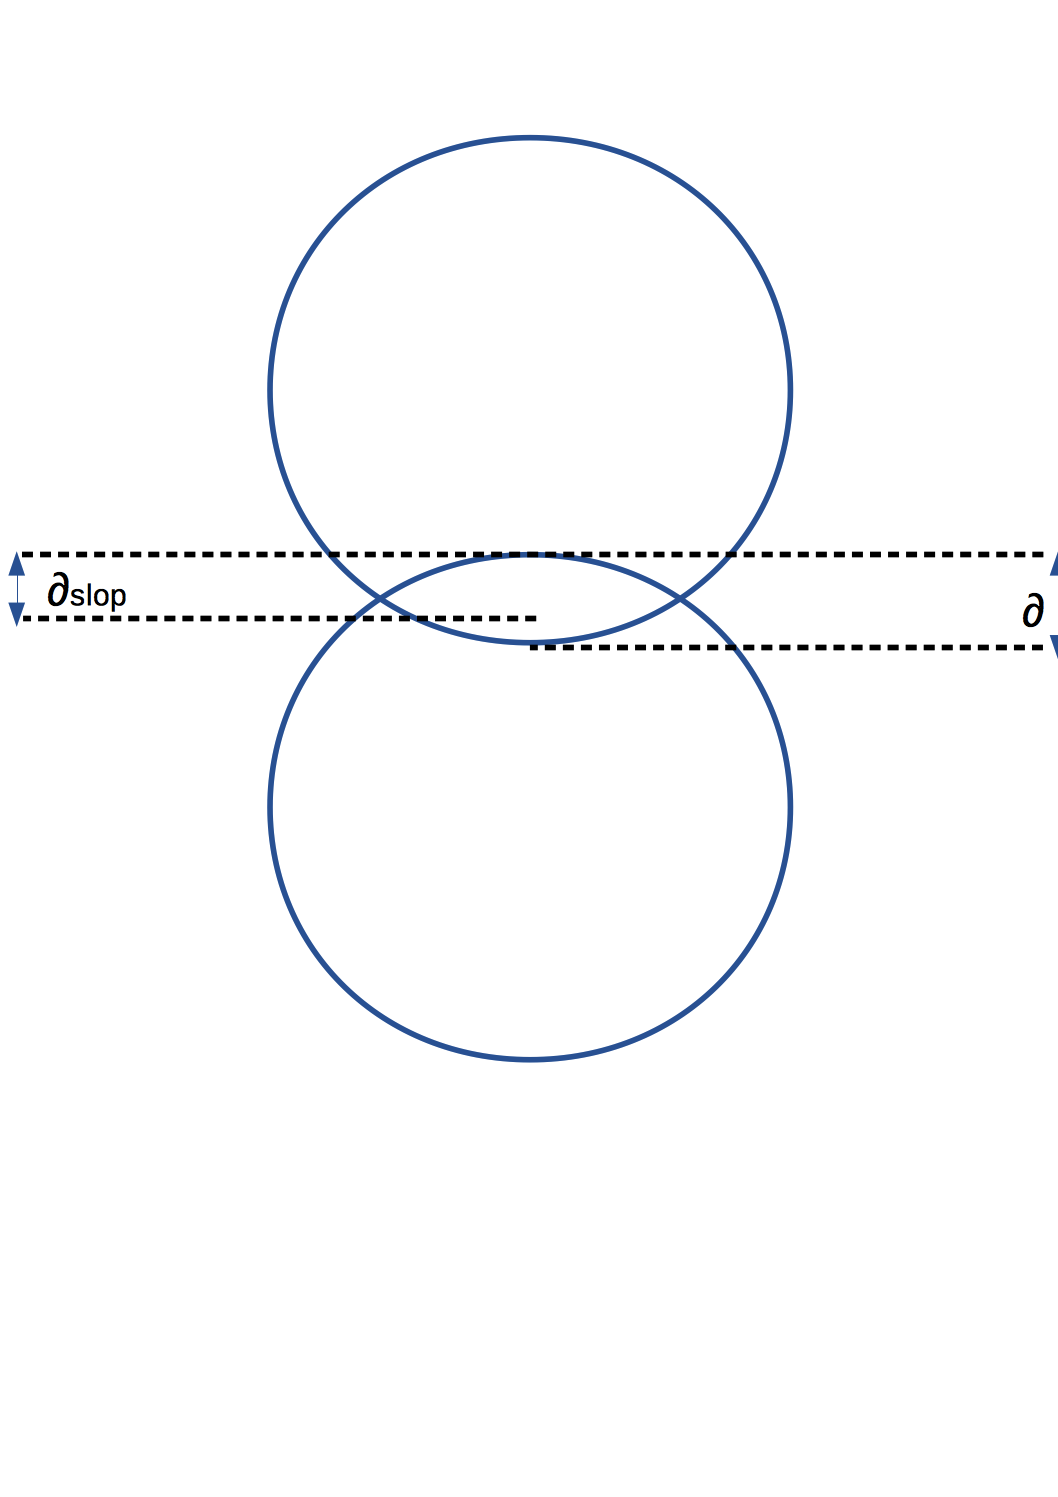
\includegraphics[width = 0.4\textwidth]{slop.png}
  \caption{Diagram of the relevant vectors and variables used when determining $\delta_{slop}$ and
  overlap. The figure is gathered from the presentation by~\cite{catto2006}.}
  \label{fig:slop}
\end{figure}

\begin{equation}\label{eq:v_bias}
  v_{bias} = \frac{\beta}{\Delta t}max(0, \delta-\delta_{slop})
\end{equation}

In equation~\ref{eq:v_bias}, selecting $\beta$ between 0.1 and 0.3 are reasonable values according to~\cite{catto2006}.
With this, equation~\ref{eq:j} is modified to read the following.

\begin{equation}\label{eq:finalJ}
  \vec{j} = \frac{-(1+\epsilon)\vec{v}_{rel,\vec{\hat{n}}}-v_{bias}}
  {m_A^{-1}+m_B^{-1}+\vec{\hat{n}}\bullet(\vec{I}_A^{-1}(\vec{r}_A\cross(\vec{\hat{n}}-\mu\vec{\hat{t}}))\cross\vec{r}_A
  +\vec{I}_B^{-1}(\vec{r}_B\cross(\vec{\hat{n}}-\mu\vec{\hat{t}}))\cross\vec{r}_B)}
\end{equation}

\subsection{Inertia matrix}
To be able to simulate the rotations of the objects properly we need the inherent
property of the object to resist rotation, the inertia tensor.
In 2D this is simply a single value, at least when considering rotation around
the center of mass. However, in 3D we instead use a $3x3$ matrix called the
inertia tensor. According to~\cite{ragnemalmscream}, when the objects initial
position is aligned with the objects principal axes, we can always write the inertia tensor
as a diagonal matrix.

By voxelizing the object for which we seek the inertia tensor of and treating each voxel
as a point mass during the calculation, we can sum over all the point masses and reach
an approximation of the inertia tensor. The method is described in
 'So How Can We Make Them Scream' by~\cite{ragnemalmscream}.
$\vec{j}$ can be calculated as following.

 \begin{equation}
  \vec{J} = \sum_i
  \begin{bmatrix}
    m_i(r_{iy}^2 + r_{iz}^2) & -m_ir_{ix}r_{iy} & -m_ir_{ix}r_{iz} \\
    -m_ir_{ix}r_{iy} & m_i(r_{ix}^2 + r_{iz}^2) & -m_ir_{iy}r_{iz} \\
    -m_ir_{ix}r_{iz} & -m_ir_{iy}r_{iz} & m_i(r_{ix}^2 + r_{iy}^2) \\
  \end{bmatrix}
 \end{equation}

 This method gets quite
 good results but relies on how finely decomposed the object is.
 Below is a comparison of theoretical versus approximated inertia tensor of a cube.
 Only one of the three diagonal components are presented since the object is symmetrical
 along all three axes, thus the inertia tensor will have the same value along the diagonal.
 One can note that the inertia reaches a reasonable approximation quite quickly.


 \begin{figure}[H]
   \centering
   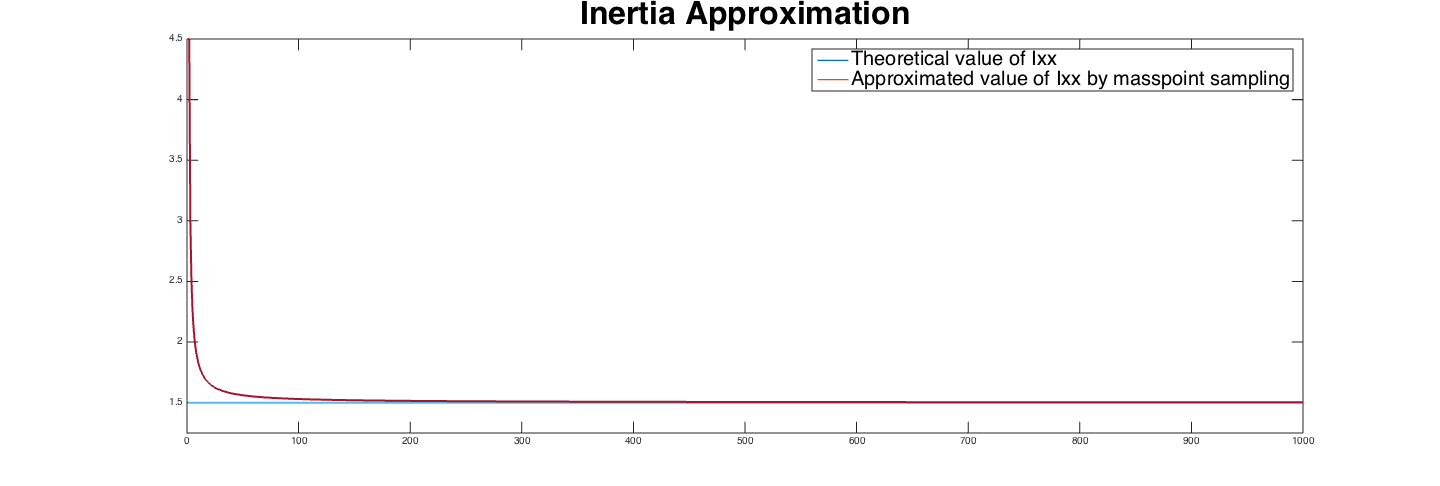
\includegraphics[width = \textwidth]{approximateIntertiaBoxSide3.png}
   \caption{Theoretical inertia versus approximated with increasing amounts of voxels.}
   \label{fig:appInertia}
 \end{figure}

% \section{Shock propagation}
% To be able to simulate a N-sphere long Newton cradle on can implement N-substep
% shock propagation. By impulse solving and updating the velocities but not the
% positions one can transfer the impulses N bodies away from the original impact.
% This works since all spheres in the cradle are in collision, but the negative
% (or zero) approach velocity stops the calculation of an impulse. However, if we
% calculate the original impulse and apply it to the velocity and reiterate a new
% collision becomes valid. The method can however only propagate the shock by the
% number of sub iterations allowed and the method can become somewhat expensive.
% Using narrowphase algorithms which are not predictive (as in projects the speed)
% and reusing the same collisions detected in each sub iteration saves a lot on
% performance. This whole algorithm is described, in short, in~\cite{lembcke}.
% Pseudocode for this is provided below. Notice that no new collisions are detected.
% \begin{algorithm}[H]
%   \begin{algorithmic}[1]
%     \State DetectCollisions
%     \While{iterations < subIterations}
%     \ForAll{collisions}
%     \State calculateImpulse
%     \EndFor
%     \State applyImpulses
%     \State updateVelocities
%     \EndWhile
%   \end{algorithmic}
% \end{algorithm}
%
% Maybe have this section?
% \section{Bullet Solver}
% \section{Bullet Broadphase}
% Bullet physics as most physics engines use a broadphase algorithm to narrow down
% the potential collisions which need to be handled by the solver. Early exclusion
% can reduce the problem from $O(N^2)$ to a reasonable $O(N)$.
% One of the methods that bullet provides is the so called Sweep-and-Prune (SAP),
% sometimes known as Sweep-and-Sort~\cite{gpugems}
% \subsection{Sweep and prune}
% Each object in the world is assigned an AABB (Axis-Aligned Bounding Box) and these
% boxes are then projected unto each of the axes X,Y,Z. A pair of boxes can have a
% potential collision if and only if the pair overlap on all axes
% (see separating axis theorem in for instance~\cite{ragnemalmpolygons}).
% The projection is a reduction in dimensionality which give a significant performance increase.
% In addition one can optimize the algorithm with some intelligent design decisions
% concerning array handling and keeping the arrays sorted. The details are quite nicely
% described by~\cite{SAPPierre} and is left up to the reader to peruse. \cite{bulletPipeline}
% talked about a parallel implementation of SAT during his talk at GDC.

  \chapter{Bullet Rectangle Bounding Box}\label{cha:meth}
For this thesis a comparative evaluation was decided upon, for that a baseline is
required. I decided on a rectangle bounding box around the model
as a simple method to compare against. It has obvious shortcomings in all
areas, except maybe, performance.

\section{Implementation}\label{sec:recImpl}
An axis-aligned bounding rectangle is fitted around the model.
Bullet includes a collision shape for rectangles and these rectangles can be used
to represent the ground plane and the bin itself, i.e. the world.

Bullet 2.83 is used to simulate the rigid body system.
Bullet's sequential impulse solver is used to simulate the system. The broadphase
was set to AxisSweep3, with a simulation world as large as the bin, with some margin, in the
xz plane and thrice the height of the bin for y, as the models are initiated in a stack
above the bin. This height could easily be calculated and set to fit snuggly instead.
However, using the same world size for each simulation gives more comparable time measurements.

In figure~\ref{fig:startStack} the initial distribution of the models is visualized.
The models are placed in a stack spaced as to not intersect, and shifted with a random
offset in the xz-plane to inject some chaotic behavior in the final distribution.
The final state of this simulation is visualized in figure~\ref{fig:stopStack}
without bounding boxes rendered and with bounding boxes rendered in figure~\ref{fig:stopStackBoxes}.

\begin{figure}[H]
  \centering
  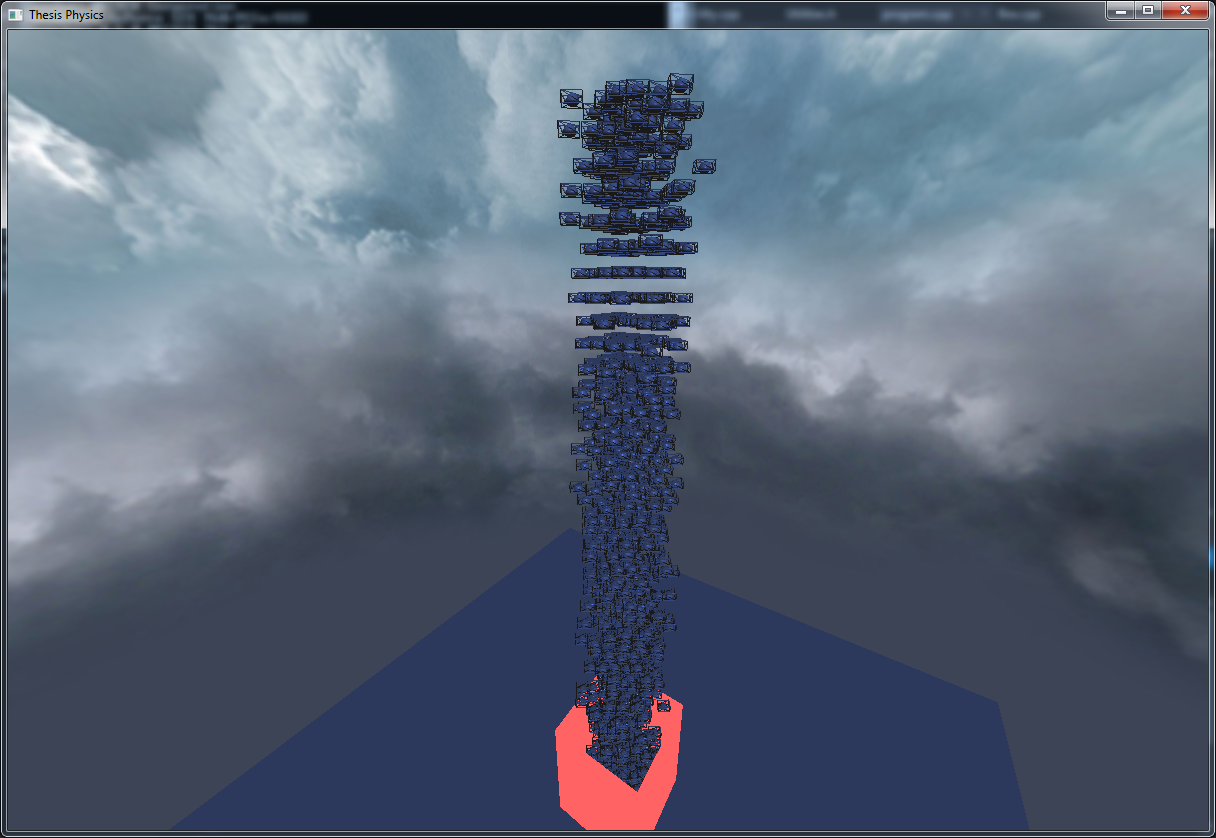
\includegraphics[width = 0.8\textwidth]{Screenshots/startofSimulation1000bodies01-22(Bugged).png}
  \caption{The start state of the simulation. Models are stacked with some margin in between and translated by a offset in the xz plane randomly. }
  \label{fig:startStack}
\end{figure}

\begin{figure}[H]
  \centering
  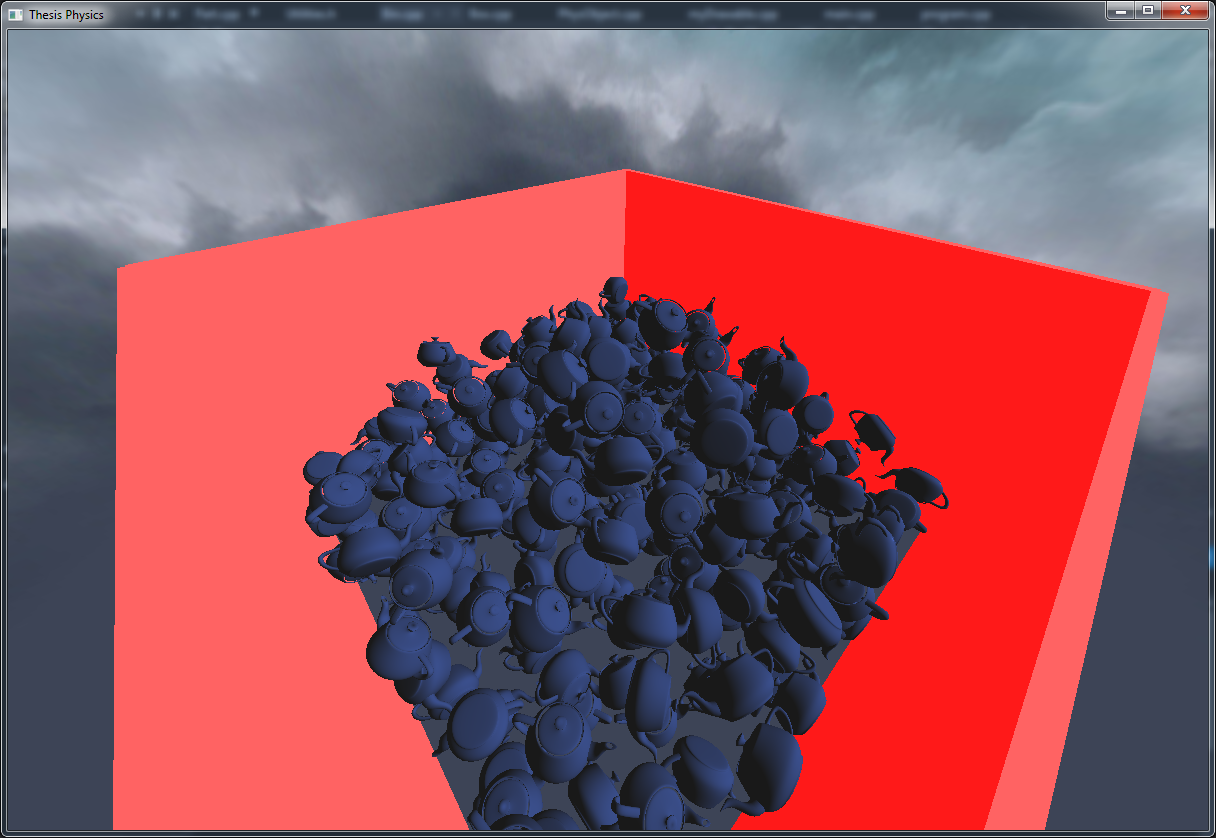
\includegraphics[width = 0.8\textwidth]{Screenshots/bulletBoxNoWire01-20(Bugged).png}
  \caption{The final state of the simulation.}
  \label{fig:stopStack}
\end{figure}

\begin{figure}[H]
  \centering
  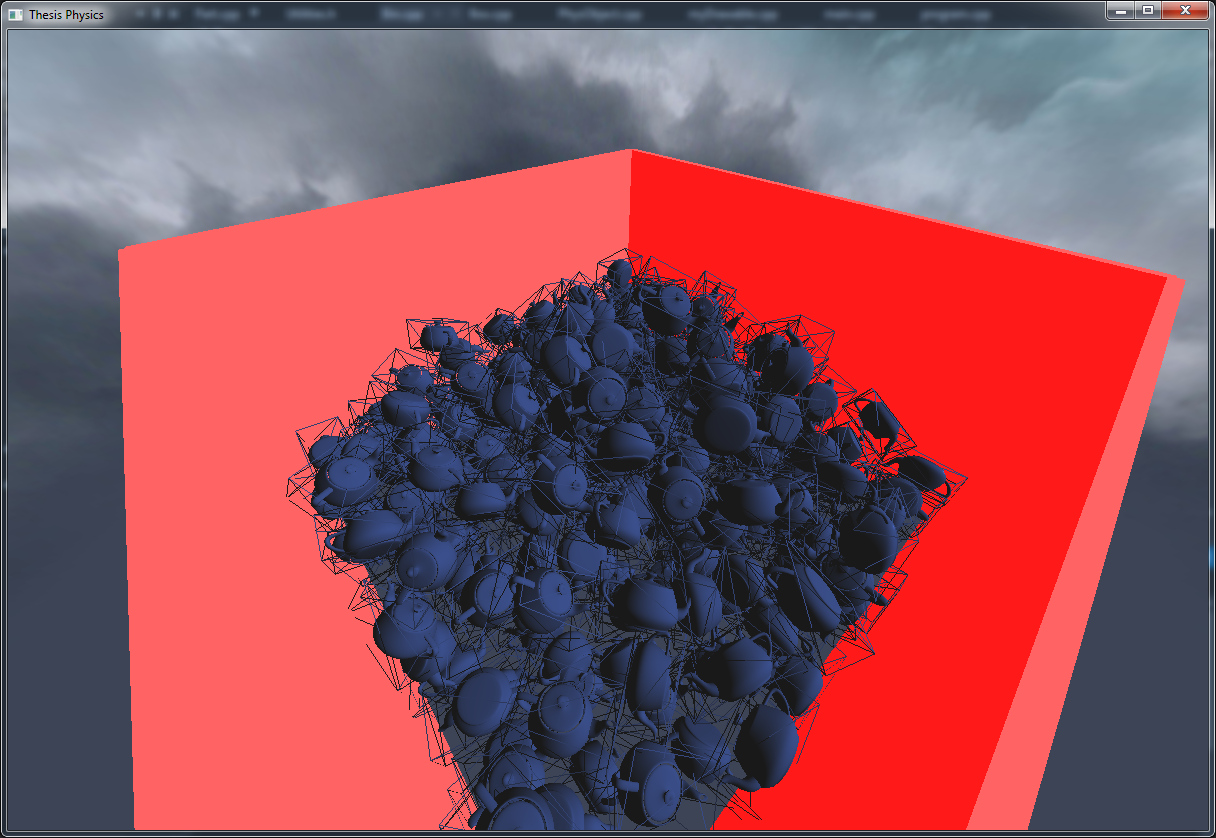
\includegraphics[width = 0.8\textwidth]{Screenshots/bulletBoxWithWire01-20(Bugged).png}
  \caption{The final state of the simulations with bounding boxes drawn.}
  \label{fig:stopStackBoxes}
\end{figure}

\section{Testing}\label{sec:testing}
Different parameters were tested to see how they affect the system in terms of performance.
The different parameters get their own explanation below, the full test data can be found in appendix~\ref{app:bullet}.
The figures present total simulation time with respect to energy threshold and sub-iterations used and
frame times for the same parameters. In addition differently sized objects were tested
as the number of layers in the stacking greatly affect the simulation time.

For details on the relaxation used see subsection~\ref{subsec:relax}.
All of the testing is done with a fixed time step of 1/60 seconds. Using a less detailed
time step lead to some of the parameter constellations to never converge.
The tests were all seeded with the the same initial seed for the random generator,
as to reproduce the initial state.

\subsection{Energy Treshold}\label{subsec:relax}
Most of the simulation time happens at the end of the simulation and only small
adjustments are made. This is not surprising at all. Basically when all objects
fall into the bin they can interpenetrate somewhat and most are not in
a stationary state. When the object then moves almost the whole system receive
repercussions of that movement. These new movements shift more objects and the
system might oscillate for a while before it finally comes to rest.
Bullet puts objects to sleep when their angular and linear velocities reach certain
thresholds, these thresholds can be modified or we can
allow the system to finish early. In this implementation I skip Bullets sleeping
thresholds and directly measure the energy of the bodies and relax the system by
allowing the system to end a simulation when the system reaches a certain
average energy per body threshold. This threshold significantly increases the performance
of the system as the small adjustments at the end tend to oscillate quite a lot before
stabilizing out completely.

\begin{equation}
E_{avg} = \frac{1}{N}\sum_{i=0}^{N-1}E_i
\end{equation}

When the system is allowed to run to zero energy, Bullets sleeping thresholds are
used. Note that at a energy threshold of 0.1 J I have never been able
to find a visual discrepancy in the distribution of the parts. Bullet inserts an
artificial additional gap between object of 0.04 units (for collision detection purposes).
So ending the simulation somewhat early is quite safe. Setting this energy threshold
too high will give obvious issues.

\subsection{Sub iterations}
The Sequential Impulse solver uses sub-iterations to resolve interpenetrations within
a time step. The amount of sub-steps taken can influence performance and how detailed
the solution is. Erwin Coumans recommends this parameter to be set between 4 and 10. Coumans E.[2015]

\subsection{Prescale factor}
The scale factor used on the model before the system is simulated.
Smaller models act more and more as a liquid where small changes propagate further
and further since less unoccupied space exist.

\subsection{Iterations}
How many iterations it took for the system to come to rest. The system is always
advanced in steps of 100 iterations since the energy needs to be measured and it
is, while quite cheap, affecting the time measurements. By only measuring intermittently
their influence on the time is reduced.

\subsection{Time}
Total time in milliseconds the simulation took, including the energy measurement
every 100 iterations.

\subsection{End energy}\label{subsec:enden}
If a threshold greater than 0 is used there will be some residual energy left in the
system.

\section{Results}
\subsection{Prescale 0.5}
The following timings are using a prescale of 0.5. The model is reduced in size by
half in each dimension before simulation. As these measurement as relative one could
theoretically made the bin larger instead. However the important point here is when reviewing the
next test series that test series uses models half as large as this test series.
\begin{figure}[H]
  \centering
  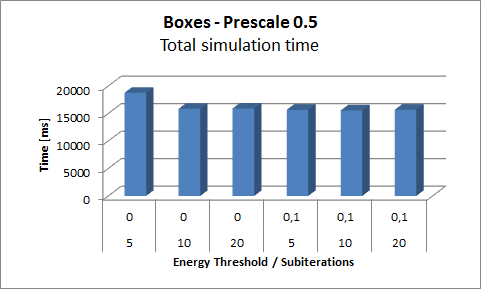
\includegraphics[width = 0.8\textwidth]{graphs/totalTimeBoxes05.png}
  \caption{The influence of energy threshold and subiterations on total simulation time.}
  \label{fig:totalTimeBoxes05}
\end{figure}

\begin{figure}[H]
  \centering
  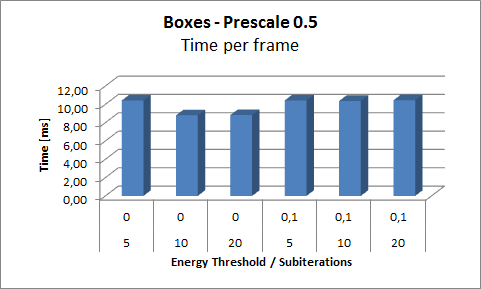
\includegraphics[width = 0.8\textwidth]{graphs/frameTimeBoxes05.png}
  \caption{The influence of energy threshold and subiterations on time per frame.}
  \label{fig:frameTimeBoxes05}
\end{figure}

\subsection{Prescale 0.25}
As previously noted, the models here are half as large in each dimension in comparison to
the previous time series, where the prescale was set to 0.5.
\begin{figure}[H]
  \centering
  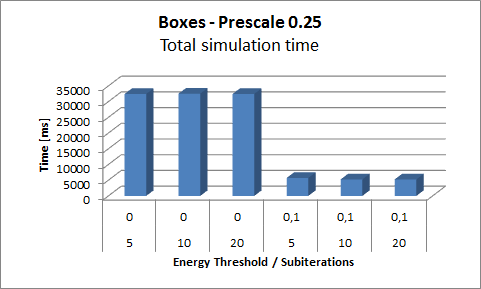
\includegraphics[width = 0.8\textwidth]{graphs/totalTimeBoxes025.png}
  \caption{The influence of energy threshold and subiterations on total simulation time.}
  \label{fig:totalTimeBoxes025}
\end{figure}

\begin{figure}[H]
  \centering
  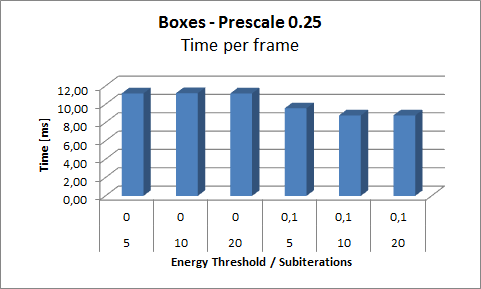
\includegraphics[width = 0.8\textwidth]{graphs/frameTimeBoxes025.png}
  \caption{The influence of energy threshold and subiterations on time per frame.}
  \label{fig:frameTimeBoxes025}
\end{figure}

An example of the end state of the simulation is given in the figure below.
\begin{figure}[H]
  \centering
  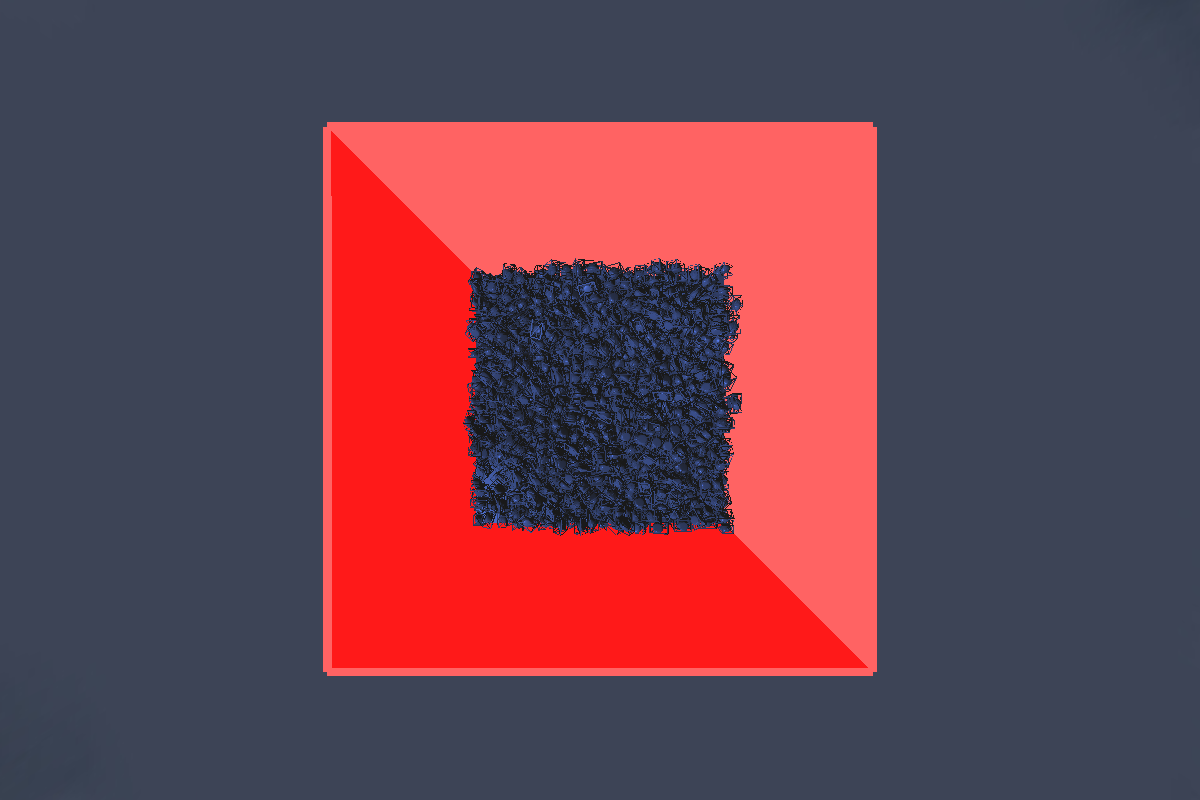
\includegraphics[width = 0.8\textwidth]{Screenshots/endState025.png}
  \caption{Finished simulation}
  \label{fig:endstate}
\end{figure}

\newpage
\subsection{Remarks}
The energy threshold saves a lot of simulation time for when the objects are small.
Small movements of a single object result in long chains of movement and the whole
system spends a lot of time adjusting at the end of the simulation state. The overall
motion at the end is small and no major adjustments are made. The early energy exit
strategy give good performance increases with small sacrifices to overall correctness
of the end state. We do not see a large performance increase for the larger models,
but the feature can, if wanted, be left activated for those scenarios as well.

The amount of sub-iterations do not seem to have a huge impact on neither simulation
quality nor simulation time.
During testing it has however been noted that selecting a very low amount of
sub-iterations, for example one iteration, could in some cases lead to oscillating,
 non-stabilizing systems. These observations let me decide on a fixed amount of sub-iterations, for
this thesis I selected 10, at the higher end of what Erwin Coumans suggests.

\section{Limitations}
One quite clearly see the limitations of this model. It cannot model concavities
at all and the collision is most of the time very unrealistic with teapots being
able to balance on their pipes, or collide with the corners of the bounding box,
where there is no model.

One could use a minimum bounding rectangle instead of a
axis-aligned one, this is however left out of this thesis as this method is not
the prime focus of the work. For reference on such methods see~\cite{minBounding}.
In addition one can quite easily by manual work rotate the model to be in a state
 which gives that the axis-aligned bounding
rectangle coincides with the optimal bounding rectangle, or at least very close
to it. For many models, such as the Utah Teapot, they are already in the optimal
orientation.

Other solvers such as NNCG and Danzig were tested as well. NNCG gave comparable
results to the sequential impulse solver. Danzig was much slower, and is by
Erwin Coumans, not suited as a solver for the whole system and should be used as
a special step in a more complex solver solution, when specific behavior is needed.
Those results are not included as this thesis is not an evaluation of Bullet itself.

  \chapter{Hierarchical Approximate Convex Decomposition}\label{sec:hacd}
Hierarchical approximate convex decomposition (HACD) can be used to decompose
concave objects into a collection of convex objects. These objects can be used
to simulate the scene instead.
\section{Implementation}
Bullet 2.83 contain a
composite (or compound) shape, a shape container which contain sub-shapes and act
as a joint rigid body. Bullet updates the inertia of the object internally as
more sub-shapes are added, as well as the bounding box needed for the SAP.

An implementation of HACD is included with Bullet's source code and the code is
developed by Mamou and based on the work of~\cite{mamou}. Some input parameters are available, these have been
left as the recommended parameters. The parameters control for instance, concavity
penalty weights, (i.e if you can disregard a small concavity)
and the maximum amount of points per convex hull.
The method while effective in terms of convex decomposition can not be described as
particularly effective in terms of performance. A Utah Teapot of around 4300 vertices,
takes approximately 25 seconds to decompose. The method is in addition rotationally
 variant, so results may vary depending on the rotation of the object which is to be decomposed.

 \begin{figure}[H]
   \centering
   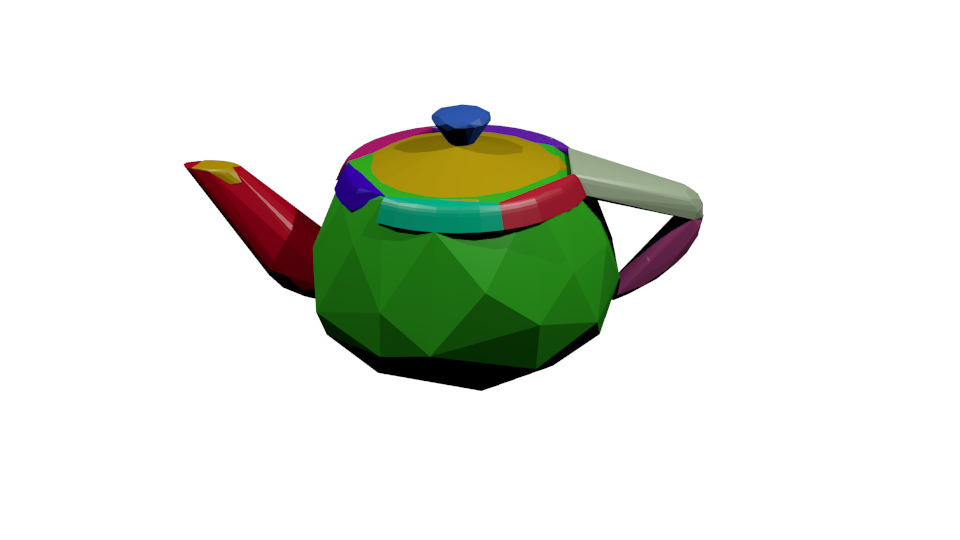
\includegraphics[width = 0.8\textwidth]{hacdTeapot.png}
   \caption{The decomposition from HACD method, model left in initial orientation}
   \label{fig:HACD}
 \end{figure}

The models are added in a three dimensional grid above the bin and the simulation
is started. In figure~\ref{fig:hacdStart} is a figure of the start position.

\begin{figure}[H]
  \centering
  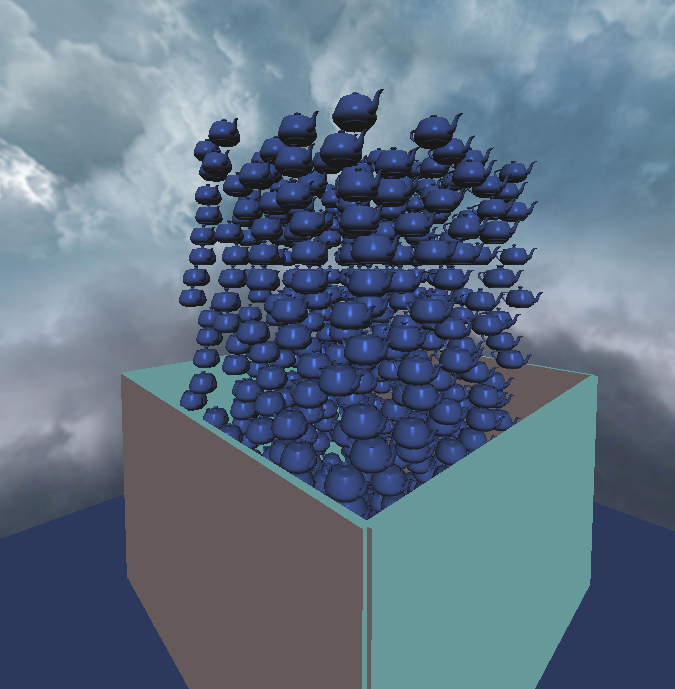
\includegraphics[width = 0.8\textwidth]{HACDstart05-11.png}
  \caption{The inital state of the simulation}
  \label{fig:hacdStart}
\end{figure}

During a simulation much more time is spent in the last
part of the simulation when most of the models are quite stationary and only small
changes are made. The increased frametime in the later parts of the simulation is
due to the many contacts between the objects. A lot of small rolling motions, likely due to the round
shape of the Utah Teapot can be observed. Without the small rolling effect Bullet's
sleeping would take effect earlier and increase performance. One can expect that
more rectangular objects will have better performance.

\section{Performance}
For testing, a Utah teapot consisting of 12 submodels were used. Each submodel have
between 50 and 100 vertices. A timestep of 0.01 seconds were used. All timings
presented are without rendering. All tests measure simulation
time and averages the result across 2000 iterations. For the first test, Bullets' sleeping was
disabled and the second the sleeping was left enabled. The results are presented
in table~\ref{tab:hacdtest}.

\begin{table}[htbp]
\caption{Testing of Bullet with HACD}
\begin{center}
\begin{tabular}{|r|l|r|l|}
\hline
\multicolumn{1}{|l|}{\textbf{Bullet HACD test}} & \textbf{Sleeping Enabled} & \multicolumn{1}{l|}{\textbf{Number of objects}} & \textbf{Time/frame [ms]} \\ \hline
1 & No & 1024 & 94.665 \\ \hline
2 & Yes  & 1024 & 78.317 \\ \hline
3 & No & 512 & 51.9156 \\ \hline
4 & Yes  & 512 & 30.5515 \\ \hline
5 & No & 256 & 22.3175 \\ \hline
6 & Yes  & 256 & 13.298 \\ \hline
\end{tabular}
\end{center}
\label{tab:hacdtest}
\end{table}


\section{Results}
The result of the simulation can be seen in figure~\ref{fig:hacd0.0} and figure~\ref{fig:tight}.
\begin{figure}[H]
  \centering
  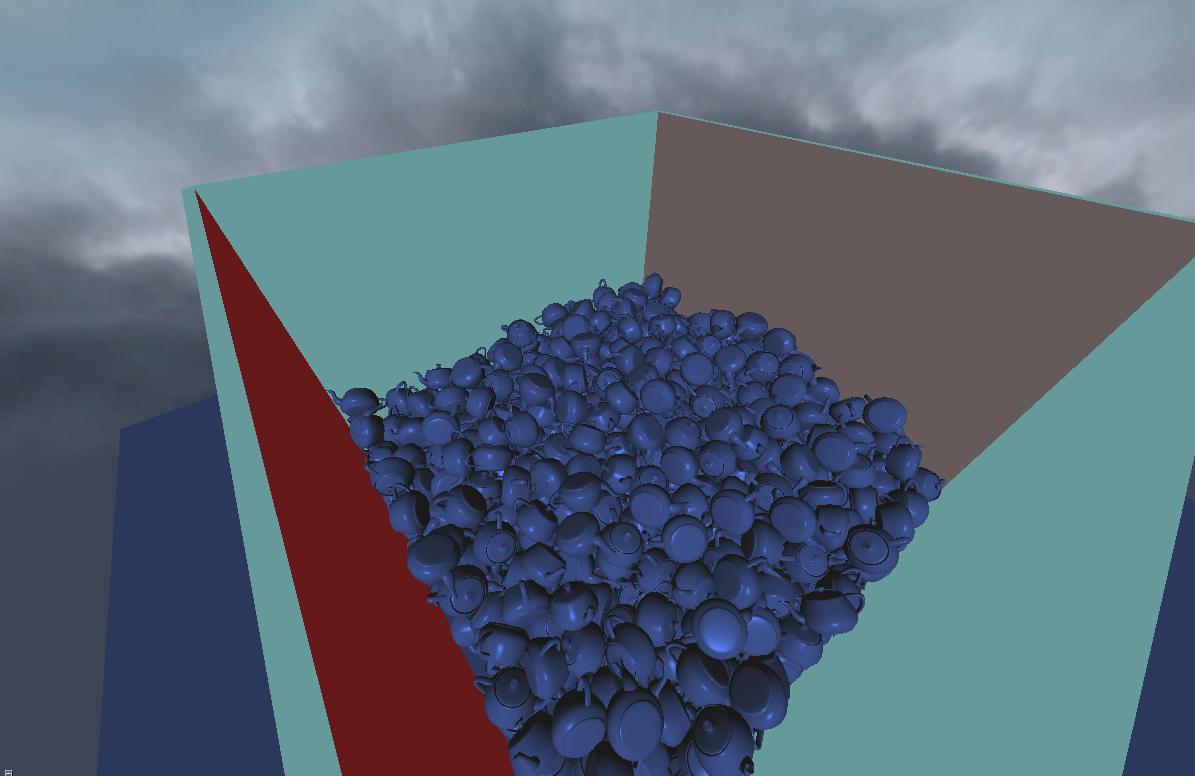
\includegraphics[width = 0.8\textwidth]{HACD512-05-11.png}
  \caption{The end result of the simulation}
  \label{fig:hacd0.0}
\end{figure}

\begin{figure}[H]
  \centering
  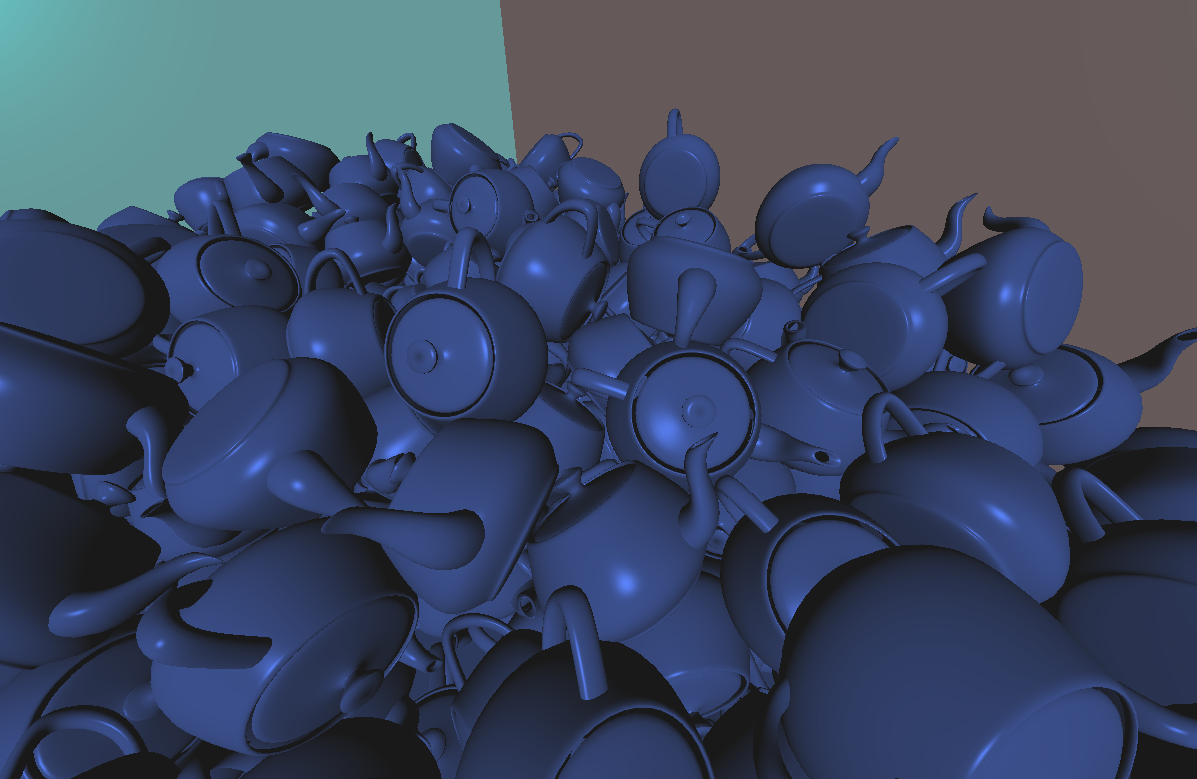
\includegraphics[width = 0.8\textwidth]{HACDtight.png}
  \caption{Close-up of finished result}
  \label{fig:tight}
\end{figure}

\section{Remarks}
While the time necessary for the decomposition renders it implausible for online uses
it is still an excellent tool for a preprocessing step, or a design step.
The models could be
decomposed at the start and copies of the same shape could be used, i.e. no additional
HACD's are performed. For this thesis the result were also saved to an Wavefront Object (.obj) file so simple and quick
 loading of the decomposed models could be used while testing.

The performance of the whole system simulation, while not phenomenal, is fast enough
for the generation of synthetic data, assuming that suitable simulation parameters
are selected.

The method does handle concave results through the approximate decomposition.

In terms of correctness the approximate decomposition, while good, does not reproduce the objects
perfectly.

%A concave collision result is portrayed in figure~\ref{fig:concaveHACD}.

\section{Limitations}
The limitations of this method are mainly concerning the performance. The fact
that the parameters of the HACD might affect the decomposition makes the system
as a whole less robust.

  \chapter{Parallel Impulse Solver}\label{cha:impl}
The parallel impulse solver will be implemented using spherical decomposition as
 described in section~\ref{sec:decomp}, using the grid based and sorted output
 collision detection described in section~\ref{sec:gridCD}. Implementation details
 concerning the collision detection can be found in section~\ref{sec:implcd}.
In this chapter I suggest solving rigid body dynamics on the GPU using spherical decomposition
however instead of using a spring-dampner model as in~\cite{gpugems} or constraint
based physics as~\cite{flex} suggests, I investigate the use of impulses.

\section{Modified Normals}\label{sec:modnorm}
Since the particles can be seen as a type of collision proxy shape for the true object,
it is reasonable to investigate what would happen if instead of the sphere's normals,
the original object's normals were used for collision resolution. For the cube only
sphere's that lies on the faces of the cube have their normals modified, the corners
and edges are left with their original normals.

\begin{figure}[H]
  \centering
  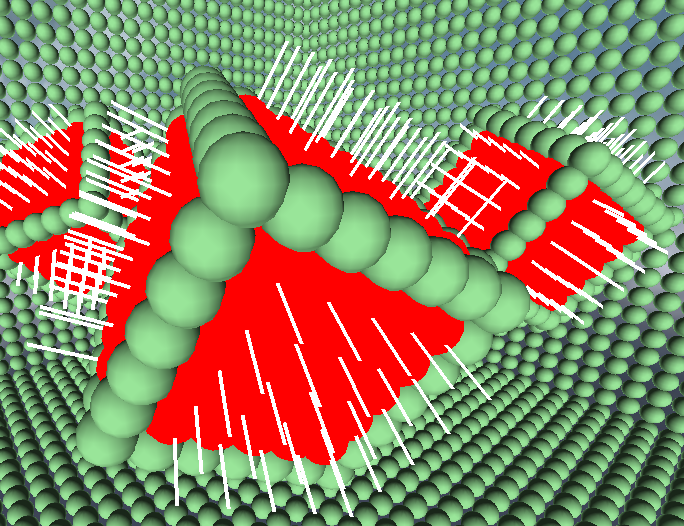
\includegraphics[width = 0.9\textwidth]{modifiedNormals04-27.png}
  \caption{Red spheres have their normals modified and the normals are rendered as lines.}
  \label{fig:modnorm}
\end{figure}

\section{Tighter voxelization}
By tightening the voxelization, while still using the same radius on the particles,
i.e. let the particles overlap within the body, we effectively change the surface
normals, overall this will lead to a smoother surface at the cost of increasing the number
of particles needed. Tighter voxelization is related to modified normals as the new
representation now more accurately models the surface and it's normals. In figure~\ref{fig:modnorm}
the spheres have been tightened and overlap.

\section{Collision matrix}\label{sec:colMatrix}
As previously mentioned in section~\ref{sec:massSplit} we need to count the collisions
between all collision pairs to acquire correct impulses. A decent way to perform
this is to keep a matrix $C$ keeping count of all collisions. $C_{i,j}$ would
contain the number of collision between body i and body j. This matrix would be
zero throughout the diagonal and symmetric. $C_{i,j} = C_{j,i}$ would
be satisfied and technically more data than required is allocated by letting $C$
be an M-by-M matrix where only M/2-M elements are required (where M is the
number of bodies). This reduction in size
has not been implemented, and instead the full M-by-M matrix is used.

A reasonable location in the shader stages for adding the collisions are during
the collision detection shader, each detected collision increments $C_{i,j}$
 through an atomic increment. A drawback of the atomic
 operations are that they may affect the performance of shaders negatively. In
 other words, the benefit that an algorithm comes with have to outweigh the potentially
 slow atomic operations.

\section{Collision Detection}\footnote{\textcolor{blue!80}{I am uncertain if this section should move to related work instead.}}\label{sec:implcd}
Initially a brute force collision detection was tested. With $O(n^2)$ it was too
slow and had poor scaling as expected. Instead the spatial partitioning with sorting
was implemented.
Each cell in the grid is $d x d x d$ where $d$ is the diameter of the largest sphere
present in the system. The grid represents 3D space and for simplicity the grid is
implemented as being $mxmxm$.

\subsection{Grid construction}
When using the sorting version of the grid construction, initially we need to count
the number of spheres in each bin and then create the exclusive prefix sum for the sorting
step. The exclusive prefix sum is calculated on the GPU as described in GPUGems chapter 39.
With the exclusive prefix sum at hand we can reset the bin counters and start the sorting.
For each sphere calculate which bin it belongs to, at the bin index check the prefix sum,
use the prefix sum as index for ordering the particles. The pseudocode below describe
the process.

\begin{algorithm}[H]
  \begin{algorithmic}[1]
  \State binIndex = hashFunc(pos);
  \State gInd = thisGlobalThreadIndex;
  \State index = prefixSum[binIndex] + atomicAdd(binCount[gInd],1);
  \State outPutSpheres[index] = inputSpheres[gInd];
\end{algorithmic}
\end{algorithm}

The hash function used for this thesis is a simple flooring of the x,y,z coordinates, a
division by the cell size ($d$) and an offset to let us center the grid over our specified domain.
Domain here refers to the coordinates which the grid covers. From $-offset$ to $xd-offset$ along the
x axis for example, where $d$ is the cellsize and $x$ is the number of bins along the x axis.
\begin{equation}
  \vec{id} = floor((\vec{p}-\vec{offset})/d)
\end{equation}

Accessing the correct bin, given m bins per dimension and $\vec{id} = [idx,idy,idz]$, becomes:
\begin{equation}
  binIndex = idx + idy*m + idz*m^2
\end{equation}

The prefix sum ensures we know beforehand how much space (or number of particles)
each bin needs. With the atomic add we can properly index into that subspace of the
array. The two following figures describe the process of sorting through prefix summation.

\begin{figure}[H]
  \centering
  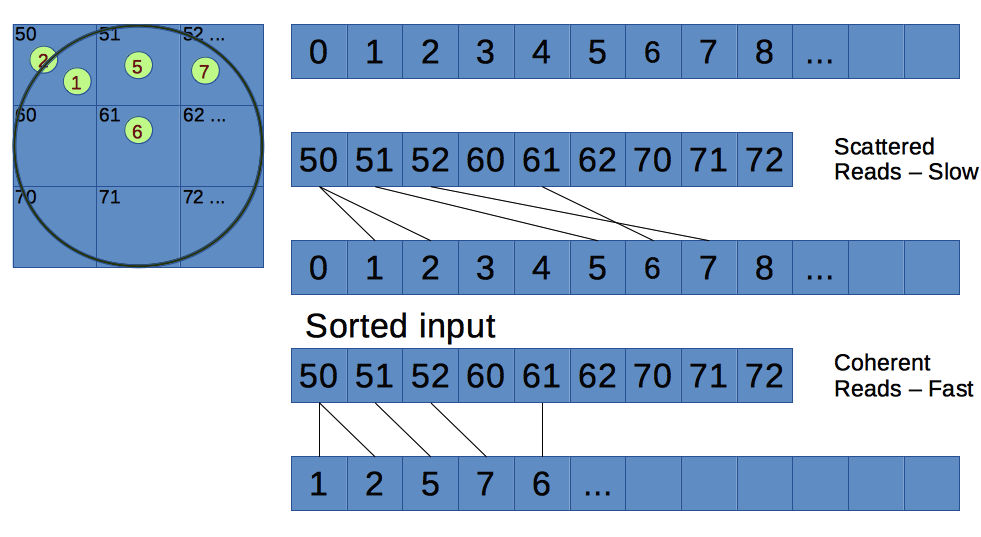
\includegraphics[width = 0.8\textwidth]{prefix1.png}
  \caption{By sorting the spheres we can get more coherent reads.}
\end{figure}

\begin{figure}[H]
  \centering
  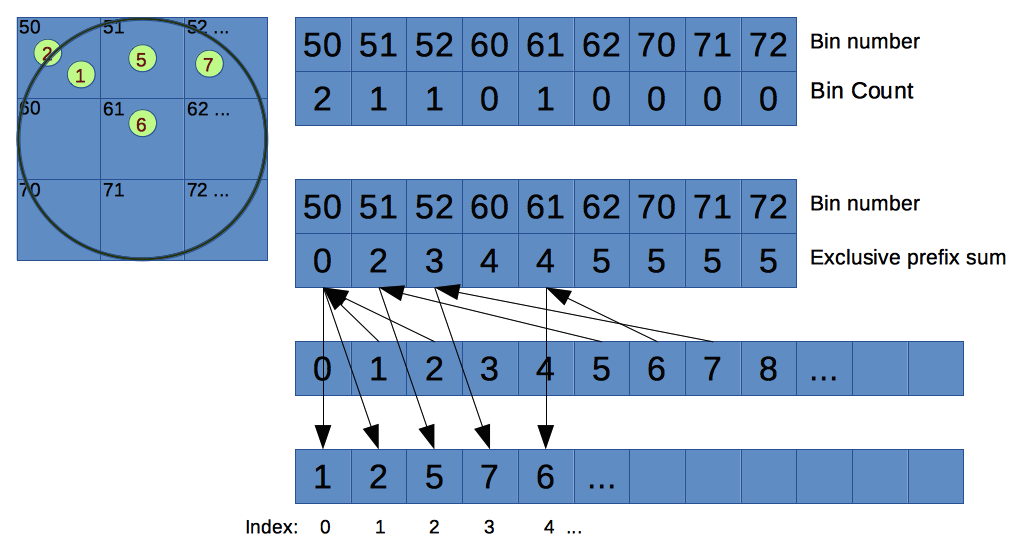
\includegraphics[width = 0.8\textwidth]{prefix2.png}
  \caption{The sorting can be performed through a exclusive prefix sum.}
\end{figure}

The overall flow of the collision detection can be summarized as below.

\begin{algorithm}[H]
  \begin{algorithmic}[1]
  \State gridCounting with atomicAdd
  \State exPrefixSum through reduction
  \State reset gridCount
  \State reorder particles with exPrefixSum and atomicAdd into gridCount to offset.
  \end{algorithmic}
\end{algorithm}

\subsection{Particles outside the collision grid}
Particles can collide even when outside the grid due to the indexing
being clamped to the grid, see figure~\ref{fig:gridStretch}.

\begin{figure}[H]
  \centering
  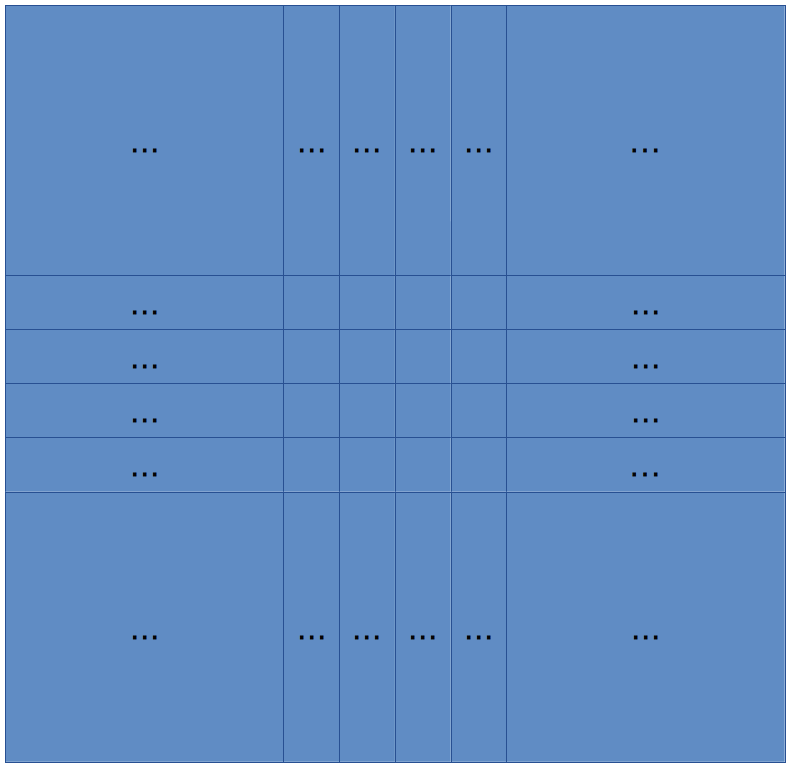
\includegraphics[width = 0.8\textwidth]{gridstretch.png}
  \caption{The cells on the edges extend infinitely due to a clamping.\label{fig:gridStretch}}
\end{figure}

However, the cells at the edges are technically infinite
in size (limited by data types) and can therefore contain a very large amount of particles and the collision
detection step may suffer greatly in performance. Consider the following two situations;
About half of the particles are initially outside the simulation domain; The grid's
cell size is doubled thus moving most of the particles previously outside into the domain, but
each collision detection will have to search through more particles.
The latter was faster during testing.

This change results in many cells containing more particles to iterate over. This was still preferable to
 letting a few cells execute slower due to containing many many more particles.
This is not surprising since this is a
parallel system. In the best case the execution time of the whole system would be
the slowest path in total through the system. This is not however always the case
since not all particles can execute in parallel.

\section{Stabilization iterations} \label{sec:stabil}
The velocity and impulse step are iterated several times to stabilize and solve
interpenetrations by a percentage of the distance as previously described.

The number of iterations needs to be high enough for the current situation, in
figure~\ref{fig:iters} is a situation where the number of iterations is too low, with the
number of iterations being 2. When too few iterations are used tunneling can occur
and in some extreme cases the bottom cubes have begun penetrating through the bin.

The spheres are assumed to be in contact however
the figure leaves some space between them for easier reading of the figure.

\begin{figure}[H]
  \centering
  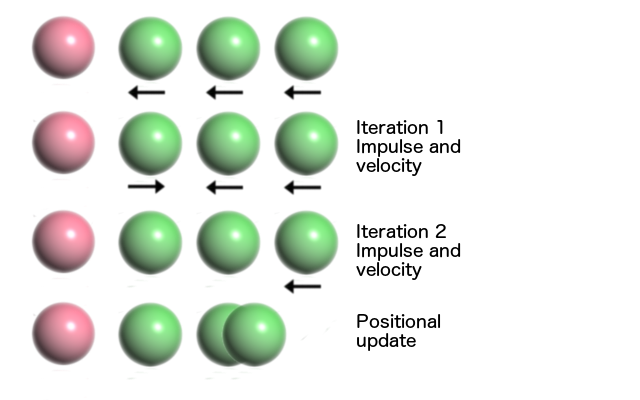
\includegraphics[width = 0.8\textwidth]{nIterationSteps.png}
  \caption{Red sphere is a static object. From top to bottom iterations increase. At the last row the positional update is visualized where interpenetration happens due to too few iterations.}
  \label{fig:iters}
\end{figure}

Unfortunately with higher stacking and increased number of objects in tight proximity,
the number of iterations needed increase or a smaller time step is needed.

\section{Shader structure}
For this implementation OpenGL 4.5 with Compute Shaders are used as the interface
for the GPU. In Compute Shaders there are several tools for workgroup synchronization
but to synchronize globally across different workgroups one need to split the program into
different shaders and synchronize from the CPU. This is done by ways of barrier bits. Global synchronization
is performed between every shader, i.e. between each box in the flow chart, in the figure~\ref{fig:flow}. Green
boxes in the figure represent shader stages which are dispatched with a thread per
sphere, whereas the blue dispatch across bodies instead.

\begin{figure}[H]
  \centering
  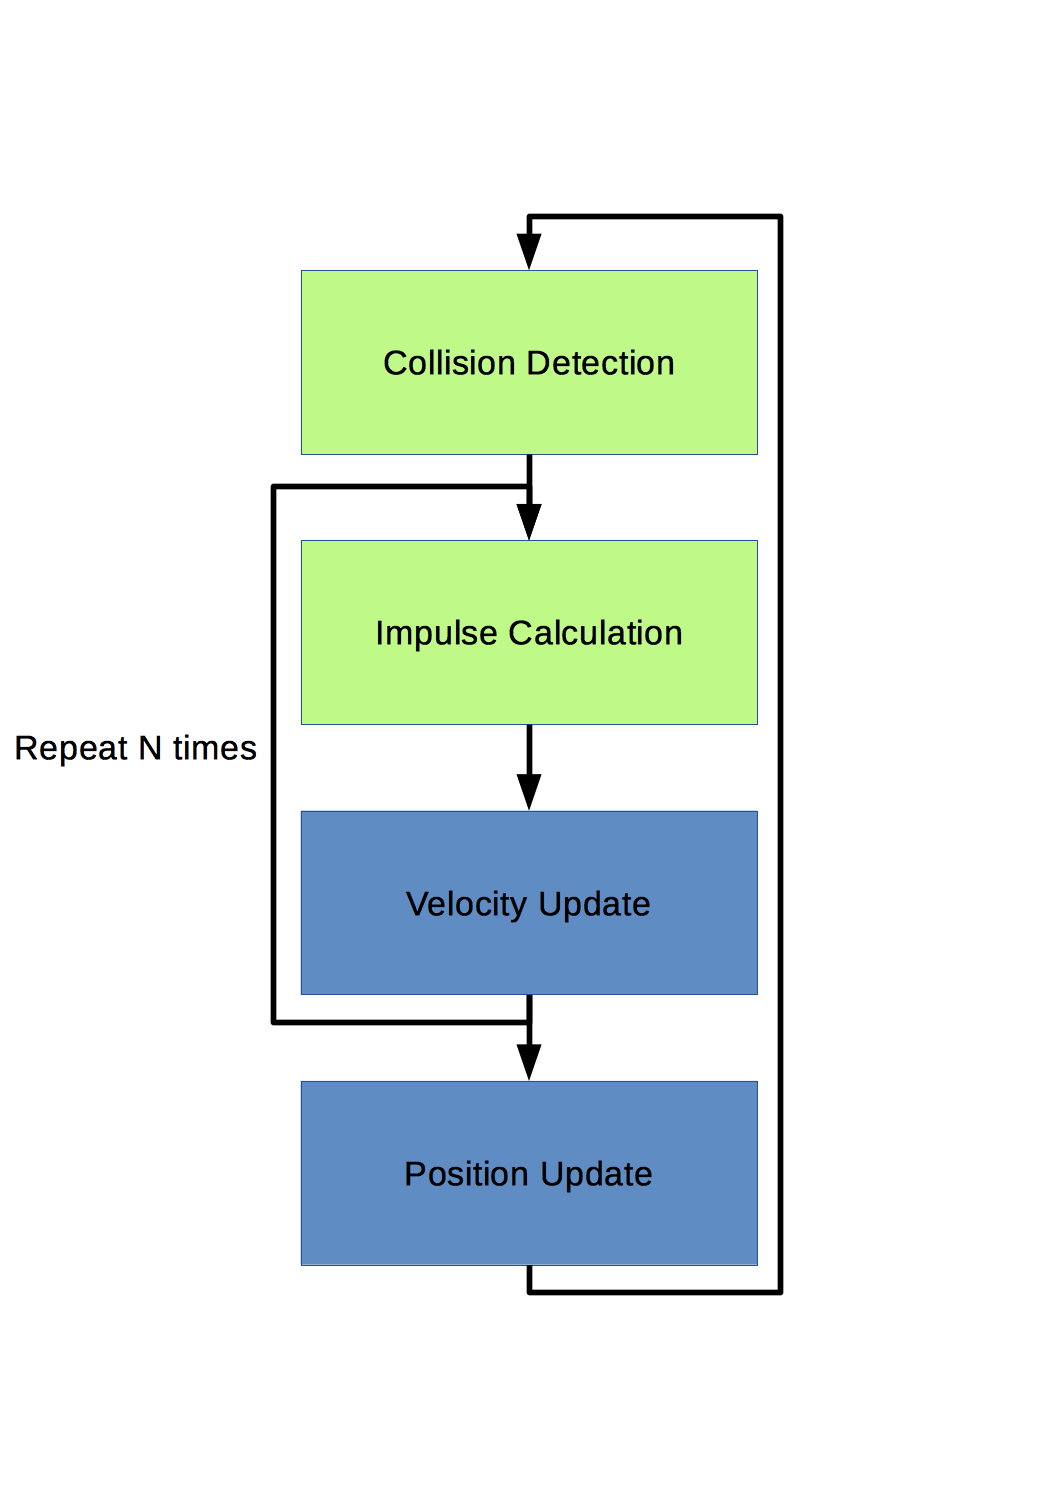
\includegraphics[width = 0.8\textwidth]{shaderflow.png}
  \caption{Flow chart of the different shaders involved. Green shaders are dispatched over spheres and blue over bodies.}
  \label{fig:flow}
\end{figure}

\subsection{Collision Detection}
The collision detection is performed through sorting and spatial partitioning.
The main problems with this approach is the limited domain which can be simulated.
The bins size should, for optimal search conditions, be exactly the diameter of the largest
particle in the system however larger bins can be used with the penalty that more
particles has to be checked. However, this results in a larger valid simulation domain.

When the collision grid and reordering is done one can find the actual collisions
among the candidates. All candidates reside in the the 26 surrounding neighboring
grid cells and the particles' own cell. The distances are measured between all
candidates and the actual collisions are saved to a contact manifold.
For this implementation a finite number of
contacts can be assigned to the manifold. For completely solid spheres eight spheres
is the theoretical maximum of contacts. However, since we use discrete time steps
the spheres could theoretically overlap and more information would need to be saved.
On the other hand most spheres have neighboring spheres in the same body which cannot
cause collisions and potentially fewer collisions could be saved. As the amount of
collisions saved affect the performance quite heavily, for this implementation a total
of four collisions are saved. This could potentially lead to incorrect results but
during all the testing no significant error could be seen.

The collisions are transferred between shader by storing them in a contact manifold.
The contact manifold contain space for the particle id of the other colliding particle,
the impulse to be applied and the normal along which we should apply the impulse.
In the current implementation the maximum amount of collisions transferred for a
particle is four. While this leaves room for error as with interpenetrating particles
more than four collision per particle can happen. Testing has shown that this happens
rarely and gives only a small impact on the outcome, it does however give a big
performance increase when transferring fewer contacts.

In the collision detection the number of collisions between body pairs is also determined.


\subsection{Impulse Calculation}
The contact manifold contain all the contacts for this sphere and the respective
id's of the spheres. For each id in the manifold read the counterpart sphere and
then calculate the impulse as described in the theory chapter. The contact manifold
also contain enough space to save the impulses and a normal direction to be used
in the velocity step. By not simply accumulating the forces in the sphere and keeping
both the impulse and the direction we can reconstruct the collision point when updating
the velocity, this becomes extra important for low resolution decompositions.


\subsection{Velocity Update}
This shader step dispatches across all bodies instead of across the particles, this
is necessary as we need to sum all the impulses from all the particles in the body.
Since no atomicFloat is supported in OpenGL 4.5, this is done through a gather scheme.
\footnote{There are ways to exploit atomic add for integers to emulate close to floating point atomic add, this has not been investigated further.}
For each particle add the influence from the current particle to the body.
Since internal particles have no influence on the simulation
those should be removed to increase performance of this shader step.
% Since OpenGL 4.5 do not always support dynamic length for loops the loop is coded
% to be very long, say 4096, and exit through a break when the final sphere of the body
% is reached.

Initially the workload of calculating the torque and linear moment was left up to the velocity shader,
this meant that fewer workgroups were issued and each workgroup had to do an increasing
amount of work and the parallelism of the GPU was utilized poorly. A new shader as
a pre-velocity step was added were the calculations for the velocity was performed
on a per particle basis and the much faster shared memory was utilized to avoid
read-write collisions. Each workgroup got a shared array with enough space to save
each particles' torque and linear moments. For the initial implementation the scaling of
the velocity step was very poor. For the tests the amount of particles in total in the
system was kept constant but the amount of particles per body was increased for each test.
This results in fewer bodies in total for each new test. The results can be seen in figure~\ref{fig:velScale1}.
For the more workload aware implementation the results can be seen in~\ref{fig:velScale2}.
As one can easily see the latter scales much more reasonably.

\begin{figure}[H]
  \centering
  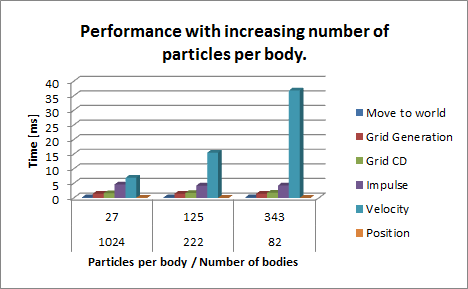
\includegraphics[width = 0.9\textwidth]{particlePerBody.png}
  \caption{Poor scaling for the velocity step with increasing number of particles per body.}
  \label{fig:velScale1}
\end{figure}

\begin{figure}[H]
  \centering
  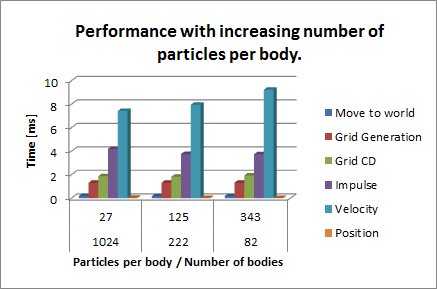
\includegraphics[width = 0.9\textwidth]{particlePerBody2.png}
  \caption{Improved workload gives reasonable scaling for the velocity step with increasing number of particles per body.}
  \label{fig:velScale2}
\end{figure}

The flowchart is updated accordingly to what can be seen in figure~\ref{fig:shaderflow2}.
The calculations performed in the velocity pre-calculation step could just as easily
be implemented into the impulse shader step instead, but has been given a separate shader
step for readability.

\begin{figure}[H]
  \centering
  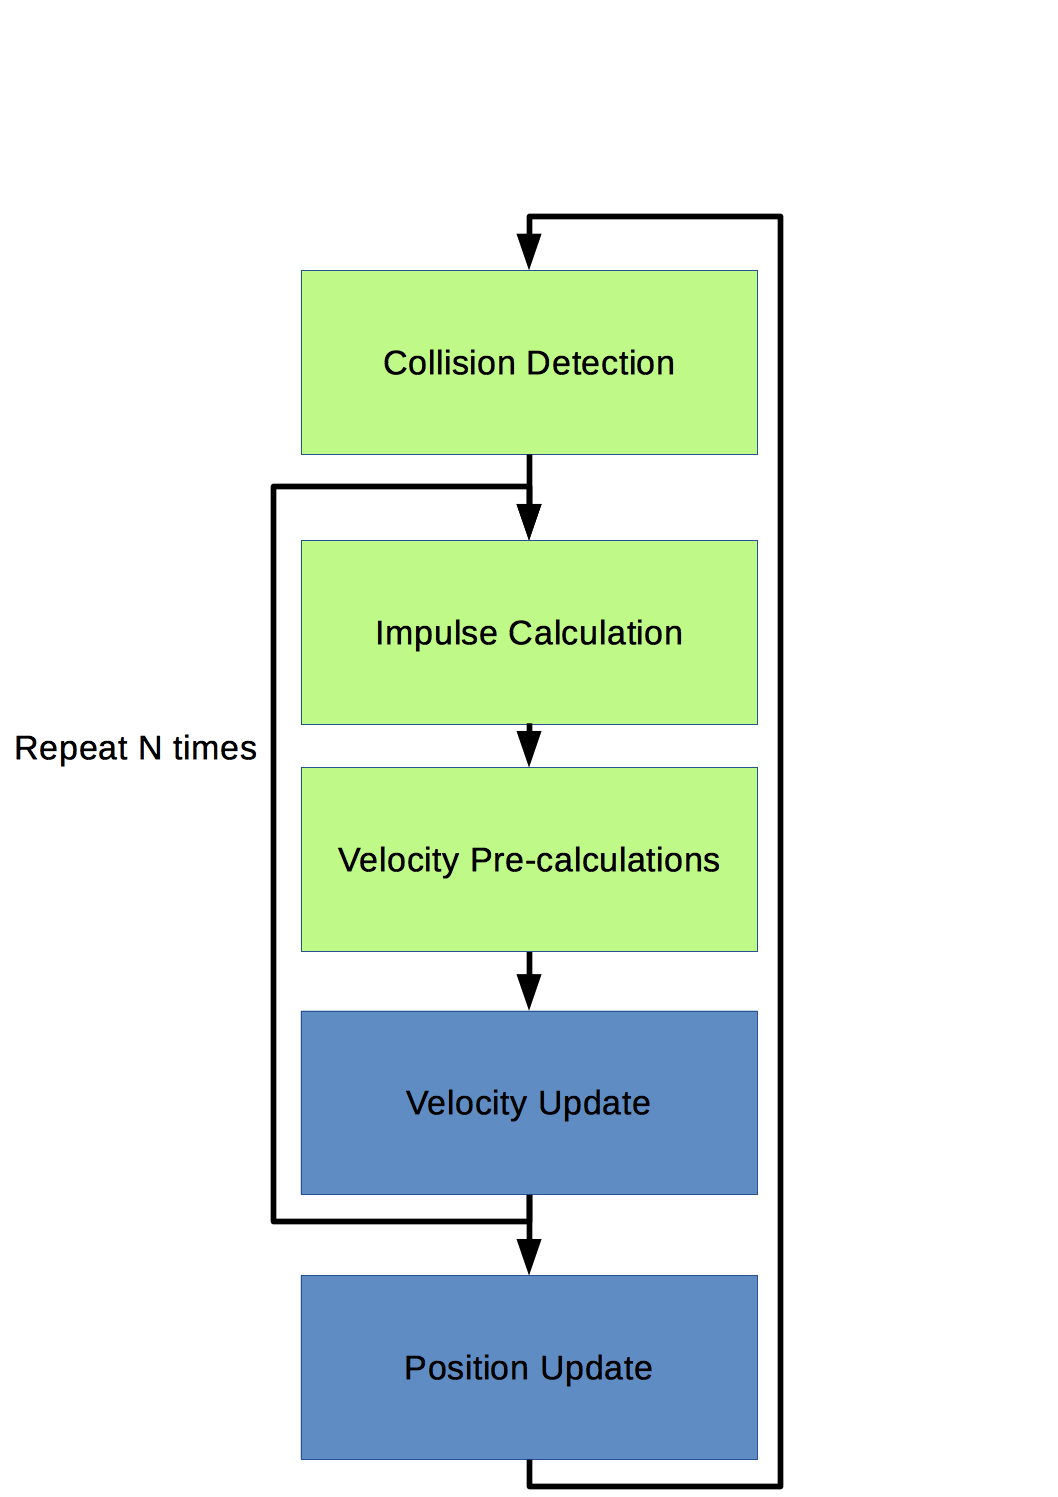
\includegraphics[width = 0.9\textwidth]{shaderflow2.png}
  \caption{Updated flow chart with pre-velocity calculations per particle}
  \label{fig:shaderflow2}
\end{figure}

\subsection{Position Update}
This shader updates the bodies' states through integration as described in the theory chapter.

\section{Optimizations}
\subsection{Impulses}
In the impulse shader we need to fetch all the other particles which have a collision
with the current particle. Prefetching these to a local variable before doing any
calculations doubled performance.

\begin{algorithm}[H]
  \begin{algorithmic}[1]
  \ForAll{particles in collision with current particle}
    Add particle to local container
  \EndFor
  \State Synchronize, ensure all threads have performed their reads
  \State Calculate impulses
\end{algorithmic}
\end{algorithm}

\subsection{Velocity update}
When calculating the forces' contributions to the velocities once again local variables
are used and synchronizations. This time the aim is two fold, one fast writes during
calculations to the local variables and coherent writes to buffer memory once all
calculations are done.

  \chapter{Results}
In the following chapter the result of physics through spherical decomposition will
be discussed and performance testing will be presented.

\section{Performance}
Since different shaders is impacted differently by different problems a few performance
test-series has been performed and will be discussed below.
For all tests, cubes have been used as the object being approximated and they
are being dropped into a bin consisting of static particles. For complete data collected and
settings used see appendix~\ref{app:test}.

The times presented for velocity and impulse (who are both iterated ten times per update)
 are the total time for all ten iterations.

\subsection{Number of particles per body}
Increasingly fine decomposition lead to more particles per body.
For this test the number of particles per body increase for each series and is
compensated by adding fewer bodies so that the number of particles in the system
in total is kept constant. For all three series some particles from the bin had to be
either added or removed to keep the total equal between the tests.
\begin{figure}[H]
  \centering
  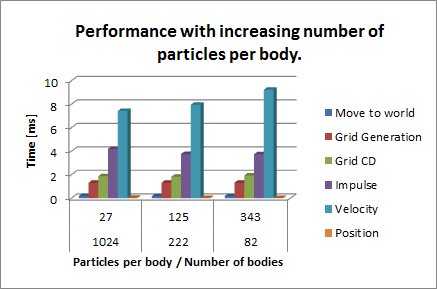
\includegraphics[width = 0.8\textwidth]{particlePerBody2.png}
  \caption{Chart of performance of each of the shader steps for increasing number of particles per body.}
  \label{fig:particlePerBody}
\end{figure}
As we can see the velocity shader time increase with the number of particles
within a body. This is not surprising as the shader performs a gather scheme for
summation of the impulses. The shader will perform a number of global reads proportional
against the number of particles in the body per thread.

\subsection{Increasing number of static particles}
For this test we let the number of static particles in the simulation increase
by increasing the dimensions of the bin (box).

\begin{figure}[H]
  \centering
  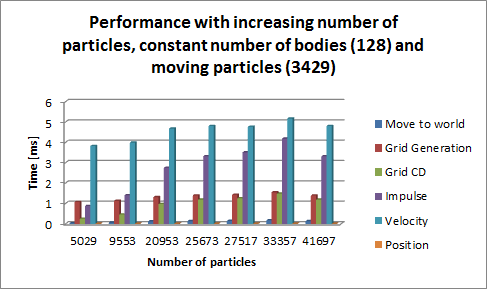
\includegraphics[width = 0.8\textwidth]{staticParticlesIncrease.png}
  \caption{Chart of performance of each of the shader steps for increasing number of static particles.}
\end{figure}

We see some time increase in the grid collision detection and the impulse calculations
and a small increase in the grid generation.
The increase in impulse is not surprising as each particle, even static ones, perform
global reads and writes per particle in the impulse shader step. One could potentially
use a early exit strategy and not perform the impulse calculations for static particles,
however, unless the whole workgroup is static particles one is not guaranteed that
it will net any performance gain as returning threads within a workgroup do not ensure
that new work can be performed.

\subsection{Increasing number of bodies and dynamic particles}
For this test we increase the number of bodies (and particles) in the system.
\begin{figure}[H]
  \centering
  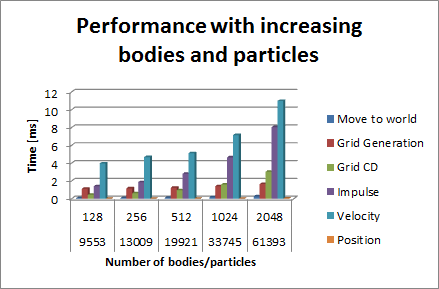
\includegraphics[width = 0.8\textwidth]{bodiesIncrease.png}
  \caption{Chart of performance of each of the shader steps for increasing number of bodies and particles.}
\end{figure}

Here we can see (while difficult to see for move to world and position) an increase in every shader step.
Worst scaling can be seen among the impulse and velocity step. Those shader steps are the two involved
in the stabilization loop and both are executed ten times each per update and optimizations
to these two steps should be prioritized in the future.

\subsection{Increasing grid size}
This test measures the performance of the grid size. For a M-by-M-by-M grid we can detect collisions
effectively on coordinates between -M/2 and +M/2 in each dimension.
\subsection{Increasing number of bodies and dynamic particles}
For this test we increase the number of bodies (and particles) in the system.
\begin{figure}[H]
  \centering
  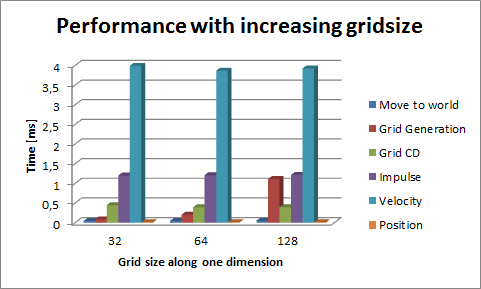
\includegraphics[width = 0.8\textwidth]{gridIncrease.png}
  \caption{Chart of performance of each of the shader steps for increasing number of cells in grid}
\end{figure}

We see that the grid generation scales poorly with the grid size, most likely cubicly
as the number of grid cells increase cubicly and the generation includes the prefix sum and sorting.
We can also note that the grid collision detection does not increase, this is expected since
we still read an equal amount of particles no matter the grid size and the particles are
sorted from the grid generation shader.

\subsection{Increasing cell size}
For this test we increase the domain of the simulation by increasing the cell size instead.
This leads to more particles having to be checked as more and more will end up in
the larger and larger surrounding cells.
\begin{figure}[H]
  \centering
  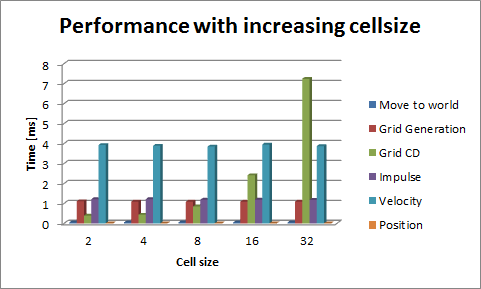
\includegraphics[width = 0.8\textwidth]{cellIncrease.png}
  \caption{Chart of performance of each of the shader steps for increasing cell size}
\end{figure}

It is only the grid collision detection shader which takes a penalty to performances
while changing the cell size, as expected. Note however that for each new series
in this test we get two times the size of the simulation domain in each dimension.
Also note that the time increase from cell size 2 to cell size 8 is only 0.34 ms in total for all shader steps.
This is cheaper than increasing the grid size from 32 to 128, which gives an increase of 0.93 ms.

\subsection{Large scale system}
With a system consisting of 1024 dynamic bodies with 218 particles per body
 and a total of 254348 particles (including
static ones), we get about 103 ms per frame, which is comparable to Bullet's HACD.
The velocity step is by far the most time consuming step, using around half of the total time with
the impulse step at a second place with about a third of the time. Once again due
to them having to be reiterated 10 times.

\subsection{Modified Normals}
Even small deviations from the sphere's normals towards the original normals quickly
led to tunneling when bodies stacked. Single bodies on a plane and similar situations
did perform reasonable. Small local changes seem to lead to the system overall not
separating the spheres properly and the idea of modified
normals seem unlikely to succeed.

\subsection{Tighter voxelization}
Tighter voxelization led to better collision result since the surface is modeled
more accurately, in addition one could decrease the number of iterations needed
for tunnel prevention and stability. This is most likely due to the reduce depth
of the indentations between particles which lead to the normals and resulting forces more often
being directed outwards from the object with a lesser angle.
 With deep indentations between particles the forces will angled more steeply and
  some of the force will not be used for separating the objects.

\section{Limitations}
\subsection{Per body particle limit}
Currently in the velocity update shader there is a for-loop across all the spheres
belonging to the current body, this is done to gather all the forces from the spheres.
To ensure performance on the GPU one uses unrolling, i.e. the for-loops content is
duplicated for as many iterations as necessary. However on the GPU this mean two
things, we have trouble with dynamic length on the for-loops and there is a upper
bound on how many iterations that are allowed. For the hardware used for the thesis,
this limit is 4096. Therefor the method is currently limited to a maximum of 4096
spheres per body.

\subsection{Tunneling}
Tunneling can occur in the system as no protection against the phenomenon is implemented.
For linear movement such a protection is easily implemented, however with rotations
the protection is slightly more difficult to implement properly. For long thin
objects a smaller time step is recommended.
\subsection{Limited domain}
In addition the domain of the simulation has to be determined before the simulation start
as a uniform spatial partitioning grid is used for the collision detection.

\subsection{False alignment}
Since the method uses spheres as a principal shape the result has a tendency to align
with the grid. A single box consisting of 27 sphere fall on a plane, also made up of spheres
at a slight rotation. All impulses present will drift towards the cube aligning with the
plane at intervals of 90 degrees. The effect would be less apparent with less regularly shaped objects and
is remedied somewhat by friction, albeit not completely.

\section{Comparison to bullet}
\subsection{Concavity}
The method can handle concave results but the current implementations poor scaling
with increased number of particles per body result in a loss against bullets HACD.
It is difficult to not talk about performance in this section as we can get good
concavity results but at the cost of increased voxelization, which in turn affects the
performance.
The performance of HACD with Bullet 2.83 will outperform the spherical decomposition
at equivalent detail.
\subsection{Performance}
In figure~\ref{fig:frameTimeBoxes05}~and~\ref{fig:frameTimeBoxes025}
on pages~\pageref{fig:frameTimeBoxes05}~and~\pageref{fig:frameTimeBoxes025}
we can read out that Bullet can simulate 1000 boxes at around 10 ms per frame.
Spherical decomposition can simulate a box decomposed with 27 spheres at around 15 ms.
The performance is comparable at this level of detail.

Since the velocity and impulse shader steps are iterated
several times for stabilization these steps are quite vital to the performance
of the method. More work could be spent on improving the performance of these shaders,
but one should also investigate if the stabilization iterations could be exchanged for
shock propagation. A sign that this might be the case is the results achieved by~\cite{flex} with nVidia Flex.

For a comparison with HACD, with bullet coming in at 100 ms it now becomes
a question of how many spheres are needed to represent our chosen object.
As presented we can simulate 1024 bodies of 218 particles at 100 ms, which is comparable to
 the implementation Bullet's HACD for 1000 bodies in terms of time. The question is
 if the results are good enough at 218 spheres which is dependent on object detail
 and required detail preservation.

\subsection{Correctness}
Correctness for spherical decomposition depend highly on how finely the model is
decomposed, much like how Bullet's HACD depends on how many vertices is allowed
per model. Boxes with as low as 27 particles looks convincing, but e.g. a Utah Teapot
may need many more particles to produce convincing results.


  %\chapter{Suggested literature}\label{cha:lit}
The following sources have been perused and investigated at the time of writing
and are intended to lay the foundation and present the initial plan of attack for
the problem.

\begin{itemize}

  \item flex, Matthias Muller et.al \newline
  A promising new technique from Nvidia. With a few exceptions the rigid body
  simulation uses the same approach as the one described in GPU Gems 3.

  \item GPU Gems 3, Chapter 29 Real-Time Rigid Body Simulation on GPUs \newline
  Voxelize the body into spheres. Solve the collisions as sphere-sphere collisions
  on the GPU. Binning the particles reduces the search time to O(n) instead of O($n^2$)

  \item Real-Time Rigid Body Interactions, Fredrik Fossum \newline
  An implementation heavily inspired by the GPU Gems 3 approach.

  \item Particle Simulation using CUDA, Simon Green \newline
  Some details on how to bin particles on the GPU.

  \item Polygons feel no pain, Ingemar Ragnemalm \newline
  For references to loads of useful 3D graphics core concepts.

  \item ...So How Can We Make Them Scream?, Ingemar Ragnemalm \newline
  Includes rigid body animation, Stencil buffers, GPGPU basics, quaternions and
  numerical integration techniques.

\end{itemize}

The following sources below are more leaned towards Bullet Physics. Bullet Physics'
experimental version 3.x include a GPU version of Rigid Body simulations which
might solve the problem very well. This would be interesting to investigate and
compare to the method(s) in the sources above.

\begin{itemize}

  \item GPU Rigid Body Simulation, Erwin Coumans \newline
  GDC presentation concerning BulletPhysics RigidBody GPU pipeline.

\end{itemize}

  %\chapter{Avslutande kommentarer}\label{cha:conclusions}
%
Sätt av ett kort kapitel sist i rapporten till att avrunda och föreslå rikningar för framtida utveckling av arbetet.


  \part*{Appendix}
  \appendix
  \chapter{Test data}\label{app:test}
  \includepdf[pages=-]{test.pdf}



  \backmatter

  \nocite{*}
  \bibliography{IEEEfull,myrefs}



  \printindex



\end{document}
